% -*- root: These.tex -*-

\subsection{Les conséquences du tournant explicatif des années 1970 sur la Validation}
\label{ssec:transition_annee70}

\subsubsection{Quelle réalité dans l'application de la démarche explicative néo-positiviste}
\label{sssec:realite_neopositiviste}

Au travers de plusieurs remarques, on questionne ici cette idée d'une modélisation en géographie faisant appel au seul cadre explicatif proposé par les néo-positivistes. On constate de façon objective l'échec de la philosophie logique néo-positiviste comme projet réaliste pour l'explication, l'inadéquation des démarches méthodologiques de géographes ayant adhérés à ce programme, trop éloignés des pratiques réelles des scientifiques, et enfin l’échec des modèles centrés sur la prédiction qui renvoient à la transformation des pratiques de modélisations.

\paragraph{Un état critique du débat épistémologique néo-positiviste}
\label{p:critique_debat}

Dès 1940 Hempel, un des membres influents dans le cercle de Vienne, s'intéresse de plus près à la problématique de la \enquote{confirmation}\Anote{confirmation} dans le cadre du modèle hypothético-déductif (la version la plus connue du modèle étant probablement la version H-D confirmatif\Anote{hd_confirmatif}). Il va alors être le premier à s'interroger \enquote{[...] non pas sur la formulation d'une hypothèse ou d'une loi universelle à partir de cas particulier, mais sur la \textit{confirmation} d'une hypothèse ou d'une loi donnée} \autocite{Lecourt2006}. Ce modèle logique va être régulièrement testé, et plusieurs paradoxes vont venir alimenter des démonstrations qui se font avant tout dans un cadre logique très formalisé. Parmis les paradoxes connus il y a celui de Goodman, ou celui d'Hempel (\textit{Raven Paradox}\Anote{paradoxe_raven} ) qui construit par ailleurs son propre modèle confirmatif \autocites{Cozic2009, Crupi2015}. Certains d'entres eux seront résolus dans différentes déclinaisons du modèle H-D, mais d'autres resteront problématiques, amenant peu à peu à l'affaiblissement de ce modèle H-D\Anote{information_confirmatif}. %l'approche cumulative empiriste.

Dans les convergences entre \textit{faillibilisme} Poppérien et positivisme logique, il existe des divergences aussi fortes que ne peuvent être les convergences. Ainsi à méthodes H-D quasi-similaires, l'hypothético-déductivisme de Popper impose pourtant un raisonnement inverse pour la formulation des hypothèses. Il ne s'agit plus d'une formulation pour la construction incrémentale de lois ou de théories, mais d'une formulation dont la fonction est avant tout de déstabiliser une théorie ou une loi existante. Pour Popper la science avance dans une perspective critique, la théorie de la relativité d'Einstein fournissant un parfait exemple de situation où le seul échec d'une expérimentation peut remettre en cause tout un pan de la théorie. Dans le langage de Popper, l'hypothèse devient conjecture, et la vérification est donc empreinte d'un double sens : une corroboration en cas d'une confrontation positive, et une falsification en cas de confrontation négative. Avec cette particularité que lorsque la conjecture est vérifiée, celle-ci est d'un apport beaucoup plus faible que dans le cas d'une vérification, du fait des nombreux paradoxes qui accablent les \enquote{problèmes de l'induction}, et que Popper veut écarter définitivement du processus de démarcation entre science et non science.

Popper, rationaliste et plus proche critique des méthodes des positivistes logiques, va proposer un modèle H-D en négatif qui remet en cause complètement l'empirisme des positiviste logiques. Celui-ci, de nouveau compatible avec la métaphysique, ne supporte plus une logique de confirmation mais de réfutation comme moyen pour séparer science et non-science.

La méthode H-D de confirmation permet de rejeter ou d'accepter des énoncés observationnels, mais elle ne constitue pas en elle-même une méthode \enquote{explicative}. La méthode Nomologique ou Déductive Nomologique (D-N) formulée par Hempel et Oppenheim est en 1945 une tentative tout à fait originale pour créer une logique formelle centrée sur l'explication.

Des discussions internes et externes de ce programme néo-positiviste s'étalant sur plusieurs dizaines d'années ressortent deux modèles en définitive compatibles, le modèle Hypothético-Déductif H-D pour la \enquote{falsification/corroboration} de Popper et Déductif Nomologique (D-N) (connu aussi sous le nom de \foreignquote{english}{covering law}) pour \enquote{l'explication} de Hempel-Oppenheim ou encore Hempel-Popper.

\blockquote[{\cite[12]{Besse2000}}]{On obtient une explication causale d'un événement (ou phénomène) lorsqu'on peut \textit{déduire} un énoncé (pronostic) décrivant cet événement. La déduction est obtenue à partir de deux types d'indications (les prémisses) :
\begin{itemize}
\item d'une part des énoncés universels ayant le caractère de lois de la nature;
\item d'autre part, des énoncés singuliers, spécifiques au cas considéré, représentant les conditions initiales.
\end{itemize}
L'explication nomologique se présente donc comme un raisonnement déductif, soit un discours d'un certain type, dont d'ailleurs Hempel a proposé [...] une formalisation. Mais, surtout, Hempel a souligné le fait que des explications de ce genre sont ce qu'il appelle des \enquote{explications par subsomption sous des lois générales}. Expliquer un phénomène quelconque, c'est pouvoir le ranger sous une loi générale, [...] une \enquote{loi de couverture} (\textit{covering law}).[...] Expliquer le phénomène, c'est être en mesure de le reformuler à l'intérieur d'un langage théorique. L'explication est identifiée avec un mécanisme logique d'inférence. Pouvoir expliquer, c'est pouvoir inférer.}

C'est aussi de ce schéma logique que dérive le concept de cause considérant l'explication et la prédiction comme équivalente.

\blockquote[{\cite[12]{Besse2000}}]{Expliquer c'est prédire. Un certain nombre de conditions dites initiales ou antécédentes étant réunies, un certain phénomène ne peut manquer de se produire, comme conséquence, compte tenu de ce que l'on sait en général des relations régulières (= lois) entre les phénomènes de ce genre.}

Il ne s'agit pas de rentrer dans les détails des critiques qui ont été faites à ces deux versions de modèles ici, tant elles ont été nombreuses, et sur ce sujet on pourra se rapporter aux ouvrages de \textcites{Chalmers1987}[214-215]{Meyer1979} et du côté des épistémologues géographes au travail de \autocite{Besse2000}. En définitive, et c'est probablement là le principal argument qui rend désuet l'appel encore aujourd'hui à une telle philosophie, les principaux acteurs de cette méthode, comme Hempel, abandonnent définitivement le modèle vérificanioniste en 1950-51, et le falsificationisme en 1965. Des dates qui illustrent le décalage temporel existant avec les tentatives des théoriciens comme Harvey d'adhérer à une telle démarche en 1969, alors qu'elles sont d'ores et déjà dépassées. Il faut également garder à l'esprit que ce sont des modèles logiques très simplifiés utilisés principalement par des philosophes logicistes, les versions que l'on rencontre dans la littérature, y compris en géographie, sont des formes plus relâchées de ces modèles \autocite{Besse2000}.


% For example, we can deduce the height of a flagpole from information about its shadow along with trigonometry and laws of optics. But it seems odd to say that the length of a flagpole's shadow explains the flagpole's height. Konolige's subset-minimality requirement serves to rule out some of the cases of irrelevance that philosophers have discussed, for example the explanation that a man is not pregnant because he takes birth control pills. But other examples such as the flagpole show that some additional notion of causal relevance is crucial to many kinds of explanation, and there is little hope of capturing this notion using logic alone.

%Parmis les défaut principaux qui paraissent poser problème pour un usage raisonné de cette méthode dans la discipline, a) il est impossible de différencier logiquement une loi d'une simili-loi, comme cela pourrait être le cas en géographie; b) le modèle D-N n'est pas universel ; c) la complétude dans l'explication scientifique est un mythe, et même si elle était possible était universellement possible, n'est pas un gage de scientificité, et inversement; c) la symétrie entre explication et prédiction n'est pas vrai; toute prédiction n'est pas explicative et inversement; c) le modèle est linéaire, une cause entraînant un effet, peu compatible avec la complexité du monde réel; d) le processus de découverte se situe en dehors de l'analyse e) la conclusion est contenu dans les premisses ; f) l'explication est en réalité plus justification, et ne rend pas forcément compte des processus générateur

%\hl{Colle pas avec la suite, soit il manque le développement, soit il faut le déplacer plus haut dessous le modele ND qui reste à détailler }
%Deux choses peuvent nous intéresser particulièrement dans ces critiques. D'une part non seulement ce modèle est loin d'être universel, et ne garantie aucunement l'explication, c'est l'objet du premier paragraphe. D'autre part la remise en cause de la symétrie entre explication et prédiction car toute prédiction n'est en soit pas explicative et inversement, et fera l'objet d'un deuxième paragraphe.

%Les faiblesses dont il sais déjà qu'elles existent : ignorance de la recherche comme activité, symétrie entre explication et prédiction, absence de découvertes autres que celle contenue dans les prémisses.

\paragraph{Les principaux instigateurs de ce cadre explicatif en géographie}
\label{p:instigateurs_mouvement}

S'il est clair que le positivisme logique n'est pas au fondement de la révolution quantitative \autocite{Claval2003}, l'impact de ce mouvement sur la géographie dans la décennie 1960-70 existe, ne serait-ce que par la portée des théoriciens qui ont bien voulu s'en faire le porte voix, cela de façon implicite comme Bunge, ou plus  explicite comme Harvey. La mesure de cet impact reste par contre difficile, sinon impossible à quantifier.

La première introduction au positivisme logique chez les géographes semble au départ se limiter aux étudiants présents sur les bancs de l'université de Washington (Seattle) et d'Iowa \autocite[554]{Barnes2001a} \autocite[120-121]{Unwin1992}, ce qui concerne aussi les étudiants en déplacement pour leurs études du fait des échanges internationaux réguliers et caractéristiques de la tradition anglo-saxonne.

Un bon point de départ pour observer la diffusion de ces méthodes semble être l'histoire personnelle de Schaefer. L'article de Fred Schaefer \autocite{Schaefer1953} est souvent désigné \autocite[15]{Louail2010} comme le catalyseur des frustrations d'une génération de géographes envers les pratiques alors en cours dans leur discipline, en déclin tant d'un point de vue scientifique qu’institutionnel.

Né à Berlin, Schaefer profite d'une solide formation inter-disciplinaire en Allemagne, qu'il fuit dès lors qu'il est apparenté à un terroriste par les Nazis, du fait de ses appartenances politiques. Après un court exode en Grande-Bretagne, il s'installe aux État-Unis où il participe à la diffusion de la géographie économique allemande, par des enseignements, mais également par le biais de traductions (Lösch) \autocite{Bunge1979}.

A la lecture de son fameux article méthodologique \textit{Exceptionalism in Geography} l'influence du programme des positivistes logiques est évidente. Rien de surprenant à cela, en effet Schaefer meurt en 1953, et c'est son ami proche Gustav Bergmann qui prend en charge la relecture et la publication finale dans les annales de l'AAG. \autocite[32]{Gregory1978}. Philosophe proche du cercle de Vienne et lui aussi exilé, Bergmann va enseigner la philosophie à la faculté d'Iowa dès le début des années 1950, tout en restant très proche et très influent auprès des jeunes géographes.\autocite[192]{Buttimer1983} Ainsi, King, Clarke, Golledge, et Johnston, sont tous passés par les bancs des universités néo-zélandaises et américaines et ont ainsi joué un grand rôle dans la diffusion de la géographie quantitative mais aussi du néo-positivisme dans ces pays. King, qui dispense des cours d'analyse spatiale à Canterbury dans les années 60 est passé en 57 à Iowa, et Golledge nous dit avoir suivi les cours de Bergman lors de son séjour dans cette même université \autocite[95-96]{Bailly2000}\Anote{new_zeland}.

L'impact premier de cet article de Schaefer est difficile à évaluer, car celui-ci ne devient un référentiel que quelques années plus tard, une fois repris par d'autres théoriciens \autocite[32]{Gregory1978}. L'ouvrage en 1962 de William Bunge, premier grand théoricien de cette \enquote{révolution quantitative}, bien que faisant une référence implicite à ce mouvement, joue un rôle important dans la diffusion de ce standard scientifique. Enseignant également à l'université de l'Iowa, celui-ci va se positionner sur la même ligne que son collègue et ami Schaefer \autocite{Goodchild2001}, et affirmer dans un article fondateur \autocite{Bunge1962} sa volonté d'une géographie avant tout nomothétique, comme les autres \enquote{sciences}. \autocites{Bunge1979, Claval2003}[429-430]{Gregory2009}.

Un autre point de vue plus tardif mais cette fois-ci explicitement teinté de néo-positivisme est réalisé par Harvey en 1969 \autocite{Harvey1969}. Bien que le travail d'Harvey soit reconnu comme un apport bénéfique à la géographie par de nombreux relecteurs (Amadeo, Gregory, Wolpert), ce travail à la fois très dense et écrit sans réel public cible en tête touche finalement une audience relativement limitée, notamment du côté des étudiants, qui disposent déjà de nombreux autres ouvrages connus comme référence (Gregory 1963, Chorley et Hagget 1965, Abler 1971) \autocite{Johnston2008}.

Connu pour son exploitation de la philosophie néo-positiviste, \textit{Explanation in Geography} est le fruit d'un travail d'écriture de longue haleine, conçu avant tout comme une position de recherche, autant de présupposés prémonitoires selon \textcite[47]{Barnes2006b} des critiques à venir. L'écriture de cet ouvrage est donc à remettre dans un contexte spécifique, en 1960 dans l'université provinciale de Bristol, ce qui fait plus de ce livre selon Barnes \autocite[31-36]{Barnes2006b} un manifeste énergique destiné à électriser la discipline, et à motiver la modernisation des institutions d'enseignement britanniques.

L'application d'une étiquette néo-positiviste à la géographie quantitative des années 1960-70 n'est pas si évidente, et une relecture plus critique de cette période permet de relever d'autres motivations, qui mettent tout autant en défaut le discours globalisant des théoriciens comme Harvey, que les discours critiques des géographes radicaux rejetant en bloc toutes les approches quantitatives.

\paragraph{Une étiquette néo-positiviste critiquée et critiquable}
\label{p:etiquette_neopositiviste}

De lecture difficile car très abstrait et mathématique, l'ouvrage d'Harvey constitue une tentative intéressante d'introduction de l'épistémologie des sciences au géographe bien qu'il reste avant tout motivé par la description d'une \enquote{démarche scientifique idéale} plus que d'une lecture rigide de l'orthodoxie prônée par les positivistes logiques. Écrit semble-t-il dans un certain isolement vis-à-vis du monde (selon ses propres termes), on comprend mieux pourquoi Harvey choisit dans son ouvrage de défendre une démarche scientifique qui sur la fin des années 1960 est déjà très largement critiquée, voire abandonnée par les autres philosophes des sciences. \autocite[147]{Ouelbani2006}. Mais en prônant cette posture délicate, Harvey s'expose tout autant aux foudres des philosophes, pour qui une attitude plus laxiste pourrait trahir la logique des démonstrations en place, que les foudres des géographes depuis longtemps enclins à la pratique d'autres types de démarches scientifiques.

%\autocite[57]{Harvey1969}

En 1972, l'ouvrage \textit{Explanation in Geography} est très vivement attaqué par une critique longue et argumentée de \textcite{Gale1972} dans le très sérieux journal \textit{Geographical Analysis}. Bien qu'Harvey présente d'autres démarches explicatives dans son ouvrage, et présente une lecture quoique superficielle, mais lucide des critiques énoncées sur la démarche néo-positiviste, il choisit quand même un alignement sur l'explication nomologique-déductive, moyennant le relâchement de certaines contraintes \autocite[39-40]{Paterson1984}. Ce qui en fait selon \textcite{Gale1972} un ouvrage propice aux débats, mais d'un autre usage limité, car cette posture de l'auteur, fluctuant autour de ce logicisme philosophique introduit de nombreux paradoxes dans l'argumentation de l'auteur.

Si l'on peut tout à fait accepter la volonté d'Harvey d'assouplir dans son argumentaire \footnote{On pensera notamment à l'assouplissement de la notion de loi de couverture universelle pour tout temps et tout espace ... } une démarche analytique de toute façon construite elle-même plus comme un idéal à atteindre qu'une réalité dérivée des pratiques des scientifiques \footnote{Cette position n'est en soit pas réellement un problème, Hempel positionnant lui-même sa méthode dans ce même idéal \autocite{Besse2000}}, il est toutefois beaucoup plus paradoxal de voir Harvey s'aligner en définitive sur le modèle néo-positiviste, une démarche scientifique analytique et réductionniste \autocite[57-59]{Paterson1984} basée sur le déroulement d'un modèle usant de causalité linéaire pour l'explication, alors que celui-ci se dit lui-même convaincu de l'éminente complexité des processus dans le temps sous-jacent à l'établissement des régularités spatiales observées et de leur importance dans l'explication.

Ainsi, dans le chapitre sur le modèle d'explication systémique de \textit{Explanation in Geography}, c'est tout à fait conscient de l'absence d'expression opérationnelle de cette méthode qu'il expose tout de même sa foi envers cette nouvelle méthode en cours d'intégration par les géographes \autocite[449,469]{Harvey1969}, en supposant que \foreignquote{english}{Whatever our philosophical view may be, it has been shown that methodologically the concept of system is absolutely vital to the development of a satisfactory explanation} \autocite[479]{Harvey1969}

Autre paradoxe, alors que seule la \enquote{loi} est censée piloter l’expérimentation dans cette démarche nomologique-déductive, Harvey admet toutefois la nécessité pour la géographie \enquote{d'une amorce} empirico-déductive, un élément important de cette révolution quantitative, ne serait-ce que parce que la géographie ne possède jusque là, il est vrai, que des lois d'emprunt \autocite[41-42]{Harvey1969}. Alors que les points de vue de Hempel et Popper convergent pour affirmer leur opposition à toute \enquote{logique de la découverte}, cette entaille au protocole avancé par Harvey n'est pas anodine. Dans la démarche de progression scientifique proposée par Hempel-Popper, la seule méthode valide pour faire le tri parmi l'infinité de faits disponibles doit se faire par la corroboration ou la réfutation d'une inférence déductive, la \enquote{théorie précédant les faits}. La formulation de l'hypothèse se fait donc \textit{a priori}, par généralisation accidentelle, ou par intuition scientifique, ce qui rend toute logique de la découverte externe au processus objectif scientifique et renvoie cette problématique à la psychologie. Une vision nettement critiquée par \textcite{Simon1973}, où il attaque largement le point de vue de Popper dans son article \textit{logic of discovery} dont il juge le titre particulièrement hypocrite compte tenu des remarques faites ci-dessus. Sans compter que les travaux pionniers \autocite{Langley2004} de Simon et Newell \autocite{Newell1961} sur les processus à l'oeuvre dans la cognition tendent à prouver qu'il existe bien une \enquote{logique de la découverte}, comme il en fait preuve avec un exemple dans ce même article.

%\hl{Floris Heukelom 2006 page 20, propos intéressant à ajouter sur SIMON 1977 et hypothèse génératives}

De plus, l'explication comme activité, ou processus en vue d'organiser des connaissances communicables n'est pas prise en compte par le point de vue des épistémologues. Or Harvey en est bien conscient lorsqu'il réalise son grand écart \autocite[10]{Harvey1969}, les géographes ne s’intéressent pas tant à la problématique de l'explication \textit{per se}, mais plutôt à son utilisation dans un contexte donné, celui du champ scientifique des géographes.

%DEBUT ORTHOGRAPHE
Malgré tout, Harvey propose une démarche de construction des modèles qui reconnaît le rôle a priori des théories sur les données, démarche qu'il oppose à la démarche classique inductive Baconienne. Le \enquote{problème de l'induction} étant ce qu'il est, irrésolu, l'inférence statistique n'est permise que dans un cadre formel orienté vers la déduction, pour la corroboration ou la réfutation d'une conjecture.

Or la critique de Popper\Anote{critique_popper} a depuis montré qu'il était possible de biaiser indéfiniment l'expérimentation pour maintenir une théorie coûte que coûte. De plus, les travaux d'epistémologues de l'expérimentation tel que \textcite[348-351]{Hacking1989} et Carthwright ont depuis largement remis en cause le rapport autrefois dominant de la théorie sur les modèles et l'expérience, faisant du modèle pyramidal d'organisation des connaissances en sciences - auquel se réfère Harvey -, un modèle de plus en plus contesté.

Enfin, le point de vue d'Harvey est étonnant quant on sait l'occasion qu'il a eu de mesurer dans ses premiers travaux l'apport que pouvait avoir dans la constitution d'une géographie quantitative une démarche empirico-inductive basée sur les statistiques (descriptives, uni ou multi-variées, spatiales). Des outils et méthodologies qui jouent un rôle historique \autocite{Pumain2003,Pumain2002} dans la capacité des géographes à construire des modèles \autocite{Sanders2000, Cottineau2014b}.

% FIN ORTHOGRAPHE
% modele

En s'appuyant sur cet état de fait, on peut mobiliser l'argumentaire de \textcite{Wilson1972} pour montrer que l'approche proposée par Harvey est bien loin de ce qui est réalisé en pratique. Celui-ci voit bien cette dualité qui existe entre les deux courants majoritaires de modélisation. D'un côté il existe cette géographie théorique issue de la branche \foreignquote{english}{Models in Geography} qui manque de données pour tester ses hypothèses, et s'avère limitée dans son expression opérationnelle (les modèles micro trop complexes, la validation et la calibration encore difficiles), et met trop l'accent sur l'induction statistique et pas assez sur la démarche hypothético-déductive pour former des modèles \footnote{Modèles est ici synonyme pour lui de théories}. De l'autre côté, la branche instigatrice des \textit{large scale models} qui fait (trop) usage des dernières techniques, dispose de larges données, mais s'avère incapable d'obtenir de bons résultats car mal équipée en termes de théorie, guidée par des objectifs divergents, où la prédiction est souvent le résultat d'un \enquote{camouflage} usant des \foreignquote{english}{Goodness Of Fit}, une technique de validation statistique alors courante en économie \autocite[10]{Batty1994}.

%Même si les problèmes d'autocorrélation spatiale, associés au \enquote{problème de l'induction} limitent effectivement la portée des généralisations qui peuvent être faites, cela n’empêche absolument pas son utilisation dans le cadre réaliste des pratiques scientifiques, et cela on imagine durant tout le processus de construction des modèles.

%\textcite{Barnes1996} produit une contre-narration intéressante sur des acteurs majeurs dans la formation de la révolution quantitative, comme Isard, Bunge, Warntz, Haggett; et prend ainsi le contre-pied de l'analyse classique plaçant la nouvelle géographie sous la seule influence d'un néo-positivisme.

Ce constat est appuyé par les travaux de Barnes qui propose une relecture critique de l'histoire de la géographie économique \autocite[122]{Barnes1996} à travers une analyse des textes et des pratiques d'acteurs importants tels que Warntz, Isard, Bunge, ou encore Haggett. C'est à ce titre qu'il affirme \autocite{Barnes2001a} le fait que bien des acteurs de la première vague théorique semblent ne jamais avoir rencontré de positivistes \autocite{Morrill1993}. Entre autre anecdote qui renforce encore ce sentiment d'une philosophie en décalage avec les pratiques, le philosophe néo-positiviste Bergman, proche des grands géographes théoriciens, n'est pas un des plus grands adeptes d'une application stricte de la \foreignquote{english}{scientific method} aux sciences sociales \footnote{Dans le recueil de texte biographique \textit{Mémoires de Géographes} \textcite[96]{Bailly2000}, Golledge revient sur les propos de Bergman : \enquote{Bergman soulignait la différence entre ce qu'il appelait alors la science pure et la science sociale. C'était le premier à admettre que l'utilisation des procédés logiques positivistes dans la science sociale pourrait se révéler extrêmement improductive.} }

\paragraph{Un échec et des critiques qui ne doivent pas masquer la réalité des transformations}
\label{p:echec_critiques}

%La problématique des modèles \enquote{a priori} défendu également par Harvey peut être en partie retrouvé dans les critiques qui sont opposés aux ouvrages et aux projets inspirés par cette démarche néo-positiviste.

Pour \textcite[41]{Gregory1978} le relâchement des contraintes préconisé par Harvey \autocite[47]{Paterson1984} autorise le développement pour la géographie \foreignquote{english}{[...] a \enquote{weaker} paradigm of explanation and theory, although one \enquote{not entirely unrelated} to the \enquote{scientific} paradigm}, paradigme basé sur \foreignquote{english}{the willingness to regard events \enquote{as if} they are subject to explanation by laws \autocite[174]{Harvey1969}}.

\Anotecontent{gregory_instrumentalism1}{Selon \textcite{Gregory1978} \foreignquote{english}{instrumentalism regards theories as devices whose utility is at stake; their truth cannot be an issue since no conclusive can be provided for them, and so science is justified in adopting a more pragmatic set of standards in whichs its propositions are evaluated to the success of their predictions and nothing else.}
}

\Anotecontent{gregory_instrumentalism2}{\foreignquote{english}{Instrumentalism plays an important supporting role in neo-classical economics, and so it is not surprising to discover that is has been carried over into much of modern geography, where its emphasis on \foreignquote{english}{goodness of fit} had had two consequences [...] First, it has allowed an extremely narrow, even superficial, formulation of spatial process to emerge, in which space-time variations are made to conforme to a typology of corresponding forecasting models. This is frequently helpul, of course [...] but the empirical identification of appropriate model structures ought not to become a substitute for the proper specification of the mechanisms involved. [...] Secondly, [...] instrumentalism has promoted a limited, at times almost an opportunist, image of geography as policy science. [...] Olsson (1972) and Lewis and Melville (1977) have shown that the instrumental approach of the social engineer dominates geography and the other regional sciences \textit{in general} \autocite[41]{Gregory1978}}}

Pour Gregory, il s'agit d'une forme d'instrumentalisme\Anote{gregory_instrumentalism1} qui renvoie la modélisation à un seul objectif prédictif, teintée d'une idéologie néo-libérale\Anote{gregory_instrumentalism2}.

Gregory fait sûrement ici référence aux résultats médiocres \autocite{Lee1973} d'une décennie de modélisation pilotée par les instituts de planification, fort coûteuse et appliquée aux systèmes urbains. Pour rappel, entre 1958 et 1968 aux États-Unis, un grand nombre de modèles théoriques \autocite[7-9]{Batty1979} dérivés des modèles de l'économie spatiale naissante sont utilisés \textit{a priori} sur de larges corpus de données, et cela à des fins de prédictions plus que d'explications. Devant cet échec, il faudra attendre plusieurs années par la suite pour que renaissent sous cette appellation des \textit{large-scale models} un tout autre programme de modélisation \autocite{Boyce1988}. % CLEMENTINE CF blog wilson

Quel exemple plus marquant peut-on trouver pour démontrer que la prédiction de systèmes aussi complexes que les systèmes urbains et par extension sociaux n'est pas compatible avec une démarche de construction des connaissances qui met sur pied d'égalité prédiction et explication ? (le fameux \enquote{Expliquer c'est prédire} de Popper).

Du côté des efforts des universitaires investis dans la construction de modèles, le livre de 1967 \foreignquote{english}{models in geography} de Chorley et Haggett encense mais cristallise aussi selon \textcite{Golledge2006} tout autant la fin que le début d'un nouveau cycle. Le peu de résultats (quelles nouvelles lois spatiales ?) apportés par des modèles théoriques aux hypothèses (volontairement ou involontairement) simplifiantes (comportement optimiseur des individus sur le plan spatial et temporel, modèle déterministe, agrégé et peu explicatif, fonctions d'utilité, population et environnement uniforme, etc.) dont on a imaginé qu'ils pourraient à un moment se substituer à la réalité, ou amener de l'explication par la prédiction \autocite[41]{Gregory1978} entraîne une large frange de géographes à critiquer dès le début des années 1970 ce type de modèle.

Si l'on oublie temporairement les assertions volontairement polémiques du postmoderniste Gregory, une partie de ces critiques semble au premier abord pertinente, et affiche clairement les dangers qu'il y a dans l'application d'une méthodologie qui tend à ignorer le mode de production des phénomènes (le Pourquoi ?), le seul moyen pourtant de donner une certaine intelligibilité aux lois que l'on utilise \autocite[14-15]{Besse2000}.

% CRITIQUE p198 science

Si on peut comprendre les inquiétudes de \textcite{Gregory1978} sur les aspects politiques et décisionnels qui découlent d'une utilisation des modèles de simulation ainsi construits (un débat encore très actuel \autocite{OSullivan2004}), son analyse ne semble pas prendre en compte les points positifs qui accompagne l'utilisation d'un tel outil. Il n'est pas fait mention par exemple de l'apport heuristique permis par les possibilités de simplification ou de complexification de l'espace avec laquelle les géographes peuvent à présent jouer pour zoomer, dézoomer ou utiliser pour confronter différentes échelles de modélisations, différents objets d'études. Des outils dont la connotation politique dépend principalement de l'exploitation qui en est faite. Malgré sa reconnaissance de l'utilité de telles constructions dans le cadre prédictif, il n'offre dans son analyse aucun futur à l'évolution de ces techniques.

Or, le rattachement des techniques statistiques quantitatives et mathématiques à une quelconque forme de positivisme est absurde ne serait-ce que parce que si on s'en tient aux catégories définies par Hacking, ou à la critique de \autocite{Dauphine2003}, le positiviste n'a que faire du mode de production de phénomènes. Ainsi, il paraît difficile de généraliser en faisant de tous ces chercheurs des promoteurs involontaires du néo-libéralisme \autocite[61-64]{Paterson1984}, ce que semble pourtant faire Gregory, en s'appuyant sur quelques citations malheureuses : \foreignquote{english}{Haggett, Cliff and Frey (1977, 517) have suggested that \foreignquote{english}{the ability to forecast accurately should represent an ultimate goal of geographical research} precisely \textbf{because} \foreignquote{english}{this ability ought to imply a fairly clear understanding of the processes which produces spatial patterns}; It ought certainly; but all the time that an instrumentalist definition of process is accepted progress is unlikely to be rapid. Instrumentalism is simply not concerned with these kinds of endeavour at all} \autocite[41]{Gregory1978} Un argument d'autant plus paradoxal que Gregory reconnaît malgré tout que cette démarche a eu son utilité (voir la citation précédente).

\Anotecontent{wilson_argument_borne}{\foreigntextquote{english}[\cite{Wilson1972}]{We must distinguish between inductive and deductive theory building. The inductive method involves theorizing from a mass of observations. In its most refined form, this is more or less coincident with statistical analysis. The deductive method involves the imaginative assembly of a theory from which predictions can be deduced; these predictions can then be compared with observation.Although the two approaches complement each other, I shall argue later that, in geography, there has been an over-emphasis on the inductive method relative to the deductive method [...] }}

Autre forme de paradoxe dans l'argumentation de Gregory, lorsqu'il appelle \textcite{Wilson1972} (un physicien !) pour appuyer son argumentation \autocite{Gregory1978}, c'est uniquement pour pointer du doigt sa critique d'une géographie qui selon lui doit plus porter sur la recherche de lois et l'hypothético-déductivisme. Or, si l'on reprend l'argumentation de \textcite{Wilson1972}, celui-ci semble tout à fait conscient que la réussite de la démarche de construction des connaissances en géographie tient avant tout de la complémentarité entre approche inductive et déductive, et appelle dans ce cadre à moins de technique et plus de créativité dans la formation des hypothèses, preuve qu'il n'est pas du tout confiné dans une approche à proprement parler néo-positiviste\Anote{wilson_argument_borne}.

Si l'on considère maintenant les géographes modélisateurs ainsi pointés du doigt, en lisant \autocites{Chorley1967, Harvey1969, Haggett1965}, on voit clairement que ces derniers sont tout à fait lucides quant aux limites imposées par l'exercice de modélisation, ainsi que de la nécessité de cerner leurs usages en fonction d'un objectif et d'un contexte. La poursuite d'un idéal prédictif peut-être un peu naïf n'enlève rien à la possibilité d'une volonté sous-jacente explicative, et cela parfois y compris quand les modèles sont réalisés pour des décideurs\Anote{lowry}.

\Anotecontent{harvey_navire}{Des théoriciens comme Bunge, ou Harvey rejoignent dans le courant des années suivantes la fronde d'une géographie radicale émergente. Ainsi \textcite[30]{Johnston2008} et \textcite[37]{Barnes2006b} nous indiquent que Harvey ira jusqu'à critiquer en partie ses propres travaux, à plusieurs reprises, dans la préface du livre, dans une réponse à son principal critique \textcite{Gale1972} et dans son nouveau livre en 1973 \autocite{Harvey1972} \autocite[166-168]{Gould2004}.}

Le néo-positivisme est un programme dont l'usage réel chez les praticiens est en réalité difficile à cerner, car on l'a vu dans le paragraphe précédent, peu de géographes se réclament explicitement de ce courant. Cette vision d'une validation des modèles basée sur la prédiction n'est pas uniquement liée aux positionnements épistémologiques de quelques individualités théoriques importantes en géographie, dont on sait comme Harvey ou Bunge qu'elles abandonnent par la suite ce navire.\Anote{harvey_navire} L'existence et la domination dans la littérature des discours de ténors de la validation comme Naylor en 1967 \autocite{Naylor1967}, laisse peu de liberté aux géographes qui ne se retrouveraient pas dans une vision de la validation avant tout guidée par l'optimisation, un biais lié à sa discipline de formation initiale en sciences de l'économie et du management. Finalement le problème semble se situer ailleurs dans l'absence à cette époque d'une part des moyens informatiques nécessaires pour l'expérimentation et la validation \autocite{Haggett1969, Marble1972}, et d'autre part dans l'absence encore d'une théorie de la validation des modèles réellement compatible avec la vision de l'explication dans les sciences sociales. Un débat qui va évoluer par la suite, avec l'arrivée de la systémique et la confrontation avec cette vision de la validation des modèles (section \ref{p:confrontation_approches}).

Autre point remarquable, l'échec de l'internationalisation de cette épistémologie est particulièrement marqué en Suède. Hägerstrand, de tradition humaniste et transdisciplinaire \autocite{Bailly2000} passe au travers des critiques car il a prouvé par ses modèles et ses outils intégrant l'homme dans l'environnement, qu'il était plus que volontaire dans la construction d'un cadre explicatif plus riche et complexe que ceux proposés alors par les macro-économistes. \hl{cf l'article belge cybergeo.revues.org\/3827} La non-diffusion en France de ce débat dans le courant des années 1970 est également à noter. En effet, Claval précise qu'il provoque au regard de l'épistémologie post-vidalienne existante un certain rejet. Le débat épistémologique intéresse certes, mais selon lui les géographes français sont alors bien trop occupés à intégrer les fascinantes et toutes dernières techniques quantitatives pour qu'une synthèse voit le jour sur le sujet \autocite[27-29]{Claval2003}.

Et quand les critiques des géographes français radicaux viennent à diviser les géographes français sur la question de l'utilisation des méthodes quantitatives, voici le type de réponse fournie par les plus quantitativistes des géographes comme \textcite[337-338]{Pumain1983} : \enquote{En effet un débat que nous considérons comme partiellement faux a beaucoup troublé la conscience de \enquote{classe} des géographes urbains. Les démarches marxistes d'une part et comportementales d'autre part, pour des raisons peut-être différentes, mais jamais très claires, ont très tôt jeté l'anathème sur l'usage de tous les outils méthodologiques et techniques d'analyse que, progressivement, l'usage de l'ordinateur a généralisés. [...] Il serait dommage qu'un tel faux débat stérilise pour longtemps une part de la géographie urbaine française, en coupant les communications entre au moins trois de ses courants les plus vigoureux. Le refus d'une approche quantitative sur un plan théorique, au profit une approche \enquote{marxisante} ou \enquote{behavioriste} autorise-t-il un piétinement méthodologique}

Ou encore \textcite[11]{LeBerre1987} pour qui \enquote{Les critiques formulées à l'encontre des traitements mathématiques et informatiques en géographie sont innombrables. Elles ont fleuri dès la parution des premiers travaux (cf. notes 10, 12 et 20). [...] D'un strict point de vue scientifique, je ne comprends toujours pas ce déchaînement sur des outils — et non sur la pratique qui en est faite — alors qu'il est prouvé depuis longtemps, toutes disciplines confondues, qu'ils sont parfaitement adaptés au traitement de certains types de problèmes.} Consciente des dérives anglo-saxonnes ou néerlandaises, Le Berre préfère souligner l'effet positif réflexif que cette confrontation a eu sur le rapport entre objets géographiques et techniques quantitatives. C'est pour elle un constat qui \enquote{ pousse à la recherche d’autres méthodes plus adéquates [...] Il n’y a donc pas d’adaptation de la géographie à la technique mais recherche d'une technique adaptée à chaque objet d'étude géographique.}

Ainsi, nous aurions tort de nous arrêter à une analyse erronée, et rejeter comme nombre d'auteurs l'ont fait toute approche quantitative, en associant à tort \enquote{révolution quantitative}, \enquote{démarche positiviste} et/ou \enquote{néo-positiviste}. Cette mise à disposition massive de nouveaux outils mathématiques et statistiques est en réalité tout à fait neutre politiquement \autocite{Sheppard2001}, et la libre utilisation de ceux-ci dans des procédures de déduction, ou d'induction tient plus de la question posée par les géographes que d'une démarche logique idéale imposée \autocite{Sanders2000}.

\Anotecontent{gregory_systemique}{Si le géographe radical Gregory semble en accord en 1978 avec la vision systémique, et dans sa force d'intégration de toutes les autres sciences dites spatiales lorsqu'il cite Chorley et les travaux qu'il réalise pour tenter de réunir l'individu et son milieu; celui-ci tout en se rattachant à un objectif nomologique, et en reconnaissant les progrès réalisés dans l'intégration des différents isomorphismes, reste toutefois très sceptique sur les premières et nouvelles applications opérationnelles dérivées de la systémique et des objectifs poursuivis comme ceux de Wilson, ou Isard :\foreignquote{english}{[...] While is it plausible for physics and theoretical biology to claim a certain universality for their concepts, the consequences of the social sciences doing so are, at the very least, extremely problematic.} \autocite[73]{Gregory1978}}

\textcite{Sheppard2001}, toujours en lutte dans les années 2000 pour gommer ce débat stérile entre géographes qualitativistes et quantitativistes, argumente en la faveur d'un langage mathématique, anthropomorphe, lui aussi vivant et amené à évoluer avec le temps pour accompagner le développement des nouvelles questions posées aux géographes.

% SUR LE FAIT QU'IL Y A UNE SYNERGIE ENTRE LES OUTILS ET LES QUESTIONS POSÉS, AJOUT SECTION SUR BENZÉCRI DONT JE NE SAVAIS PAS QUOI FAIRE ...

Ainsi, le sursaut et la transformation déjà étudiés dans la section \ref{ssec:crise_mutation} montrent que la discipline n'a pas attendu le revirement des théoriciens néo-positivistes, ou la critique sceptique\Anote{gregory_systemique} d'une géographie radicale qui explore d'autres horizons explicatifs pour remettre en question et rebondir du fait de ses propres échecs. L'évolution des mathématiques et de l'informatique permet ce dépassement, et cela au travers d'un cadre d'analyse systémique qui offre les concepts nécessaires pour sinon résoudre, au moins admettre un premier dessin de cette complexité \autocite{Dauphine2003}, avec à la clef un effet libérateur en géographie pour bien des raisons évoquées par \textcites[137]{Pumain2002}[27-28]{Pumain2003}

 % Est ce qu'il faut citer ici transformation de l'objet géographique par rapport à la technique  ? reformulation de concept, etc voir citation Denise et Berre p 13

%Intéressante aussi, la lecture du \enquote{manifeste} \autocite[31]{Barnes2006} d'Harvey donne à voir cette tension entre ce qui est pour lui la démarche dominante des années 1960-70, et l'ouverture vers un autre paradigme prometteur, celui de la systémique, selon lui encore peu repris et opérationalisé par les géographes, et cela malgré l'appel de plusieurs personnalités comme Berry, Chorley, Haggett.

%Sachant que la démarche explicative néo-positiviste proposé par Schaefer, Harvey et les autres théoriciens tient plus de l'expression d'un idéal que d'une réalité pratique, la posture nomologique sous-jacente reste quand à elle une volonté forte qui motive toujours la transformation de la discipline.  FIXME conclusion modérant les propos de rejet du courant comme principal porteur ?

\subsubsection{L'intégration progressive et naturelle du projet systémique}
\label{sssec:progressive_systemique}

La posture nomologique des géographes, en remettant au centre de son projet scientifique les modèles et la modélisation, a réactivé dans sa révolution ce besoin non pas tant d'inventer des lois spatiales \textit{ex nihilo}, car comme on l'a vu il s'agit d'un exercice qui a montré ses limites, mais plutôt d'extraire ou reconstruire en partant de ces fondements historiques la part de géographie propre à ces isomorphismes afin d'établir plus explicitement ces \enquote{lois} qui lui font défaut.

Encore dans une phase de découverte à la fin des années 60, si l'on en croit \textcite{Harvey1969}, l'esprit systémique \textcite{Ackerman1963} a déjà pourtant bien infiltré la géographie par le biais de porteurs dont le flambeau semble tout autant explicite qu'implicite à ses récents développements. Des chercheurs comme Stewart, ou Zipf-Auerbach, dont il n'est pas difficile de faire remonter la volonté d'établir des ponts entre disciplines à l'héritage des grands mouvements inter-disciplinaires systémiques du début du XXème siècle, comme la Cybernétique de Wierner, et parallèlement le programme biologique organiciste de Bertalanffy, qui deviendra par la suite le projet beaucoup plus vaste de \textit{General System Theory} (GST). \footnote{Sur ce sujet on trouvera en annexe A un historique beaucoup plus détaillé de ce mouvement.}

Il me paraît important ici de noter dans quelle position surprenante se trouvent la géographie et les géographes lorsque ceux-ci appellent à la fois à l'application d'une démarche HD/ND, et leur volonté d'aller vers une démarche systémique, tant les deux systèmes semblent s'opposer en de nombreux points (pour ne donner qu'un exemple, il faut opposer la causalité linéaire du modèle ND aux causalités multiples et bouclantes de la systémique \autocite{Besse2000}), ce qui rend leur cohabitation de toute façon relativement peu probable : approche analytique réductionniste contre holisme, causalité linéaire contre causalités multiples, etc.

Si Bertalanffy fut marqué par le néo-positivisme à une période de son étude \footnote{Fait étonnant Victor Kraft est un géographe, philosophe proche du cercle Viennois, mais tenant d'un point de vue original rapport à ce courant. Celui-ci forme des géographes très tôt en Allemagne à des méthodologies quantitatives (1929). En 1926, Bertalanffy proche du milieu viennois à ce moment, emprunte à celui-ci en 1926 la méthode hypothético-déductive \autocite[342]{Pouvreau2013}. Une boucle intéressante semble alors se former entre 1) Kraft dont la formation est inspirée par Pleck, un professeur allemand inspiré de la méthode déductive de Davis, 2) Kraft indirectement amené à participer au débat Schaefer-Hartshorne du fait de son travail ainsi cité, et 3) le fait que Bertalanffy va ensuite nourrir les travaux de Chorley qui prend la suite des études de Davis en géomorphologie...}, celui-ci subit par la suite de très violentes critiques de la part de plusieurs membres en Allemagne, puis aux Etats-Unis, marquant un profond désaccord qui ira en grandissant par la suite \autocite[26-27]{Pouvreau2006}.

Cette diffusion du projet systémique dans la géographie semble s'être faite en deux temps partiellement superposés, ce qui rend la mise en avant d'une seule et unique \enquote{rupture} difficile. Si la première phase semble plus mettre l'accent sur la modélisation et le débat autour d'isomorphismes du fait de passeurs entre disciplines, la deuxième phase plus explicite d'acquisition d'une partie du projet systémique semble quant à elle généraliser ce projet de collecte d'isomorphisme, et mobilise à l'instar des sciences physiques des outils qui bouleversent notre façon d'aborder la construction des modèles en géographie. Si la première phase introduit l'idée, la deuxième semble trouver les moyens de l’opérationnaliser.

\paragraph{Premiers passeurs et premiers débats au cœur de cette nouvelle posture nomologique}
\label{p:passeur_systemique}

Pour illustrer ce fameux thème de Norbert Elias \autocite[31-33]{Delmotte2010} \textcite{Elias1991} sur l'Homme illustre, comme produit conjoncturel des interrelations qui le portent au sommet d'une dynamique collective, on pourra citer les travaux qui mènent à la bien connue loi rang-taille de Zipf-Auerbach, en filiation directe avec cette dynamique de fond à la convergence des grands mouvements inter-disciplinaires et des nouveaux enseignements tirés des avancées physiques de la thermodynamique du début du XXème siècle.

Plus qu'une application directe souvent impossible, voire non souhaitable, ces isomorphismes semblent avant tout agir comme catalyseurs dans la transformation d'une discipline marquée d'abord par cette impression d'absence de loi. Ainsi le cas de la distribution des tailles de villes, qui se rapportent tout autant à la théorie des lieux centraux que de la loi rang-taille, est exemplaire des débats qui vont se structurer autour des modalités d'application de ces isomorphismes, et des résultats qu'il est possible d'en tirer d'un point de vue thématique.

L'interrogation sur la capacité du vivant \enquote{à remonter} l'entropie qui saisit la physique du début du XXème siècle amène Auerbach à proposer en 1910 le concept d'\enquote{ectropie} \autocite[81]{Pouvreau2013}; préfigurant ainsi les débats à venir sur cette thématique dans les années qui suivent (néguentropie de Schrödinger en 1945, second principe de la théorie organismique de Bertalanffy en 1929 \autocite[475]{Pouvreau2013}, etc.)\autocite[80]{Pouvreau2013}. Physicaliste avant tout \autocite[87]{Pouvreau2013}, Auerbach est convaincu que le progrès en biologie ne viendra que de l'explication entièrement physique des phénomènes biologiques, une vision réductionniste de la biologie qui sera largement débattue par la suite dans la thèse de Bertalanffy. Toutefois, et sur un tout autre sujet se rapportant à la physique, c'est lui qui s’intéresse en premier à l'application sur des villes de l'effet d'inégalité soulevé par Pareto dans les populations.\autocite{Auerbach1913} Il donne naissance à la loi Rang-Taille qui montre que le produit de la population par le rang de la ville dans la hiérarchie est une constante. Une analyse reprise et développée par Zipf dans une étude lexicologique à vocation universalisante, cette fois-ci appliquée sur les villes, ce qui explique entre autre la confusion dans l’historique de l’appellation.

Autre exemple d'isomorphisme catalyseur des débats, on citera parmi d'autre l'adaptation du modèle gravitationnel au modèle de migration de population. Sur les travaux initiaux des géographes Ravenstein (1885) et Levasseur (1889), puis l'économiste Reilly (1929), se greffent les travaux de Warntz (géographe) et Stewart (physiciens). Déjà connu des géographes par sa publication de 1947 qui pose l'isomorphisme entre population et gravité, Stewart fait très probablement naître une certaine curiosité chez les pionniers. Ullman s'avère par exemple être un fin lecteur \autocite[61]{Glick1988} et \href{http://nwda.orbiscascade.org/ark:/80444/xv01385}{@Correspondant} de Stewart. Warntz de son côté est un géographe qui plonge dès le départ dans l'inter-disciplinarité. Financé par l'ONR (\textit{Office of Naval Research}) il est présent à l'AGS (\textit{American Social Geography}), au département de science régionale de Pennsylvania's, et dans le département d'astro-physique de Princeton où il est amené à collaborer régulièrement avec Stewart, avec qui il \href{http://rmc.library.cornell.edu/EAD/htmldocs/RMM04392.html}{@Correspond} aussi après guerre. \autocite{Barnes2006a}.

Dans les deux cas, il est intéressant de noter le basculement manifeste entre application du modèle \foreignquote{latin}{a priori} sur les données, et la prise de conscience dans un long débat qui s'ensuit sur la faible capacité explicative de ces analogies, avec la nécessité d'adapter ces formulations à la discipline géographique, notamment en faisant appel à plus d'allers-retours entre théories et données empiriques.

\Anotecontent{Analogie_gravitationelle}{\enquote{On peut considérer que l’élaboration de ce modèle repose sur la combinaison de raisonnements a priori, d’analogies et d’observations.
Raisonnements a priori, ici, en partie très simples puisque l’on peut considérer l’hypothèse selon laquelle des flux entre des lieux sont d’autant plus forts que ces lieux sont d’autant plus peuplés et moins distants relève du simple bon sens. Le fait d’évaluer simultanément les populations en introduisant leur produit et non leur somme est moins évident a priori. Le choix fait référence à une notion un peu abstraite, qui relève de la logique combinatoire.
Le choix de la fonction de la distance résulte d’une accumulation d’observation de l’espace qui montrent bien que l’effet de la distance sur des relations n’est pas linéaire. La non-linéarité a été, ici, traduite par le recours à une fonction de puissance négative (on trouve, dans certaines formalisations, des fonctions exponentielles décroissantes).} \autocite[34]{Dastes2001b}}

Ainsi, dans le cadre de la recherche du meilleur modèle, ou du meilleur paramétrage de modèles mathématiques pour ajuster les données s'avère rapidement inutile et décevant - quand il n'est pas en plus empreint d'idéologie - tant l'apport d'un point de vue explicatif est faible. Sur l'application des modèles dérivés de l'analogie gravitationnelle\Anote{Analogie_gravitationelle}, \textcite[37]{Pumain1982} cite Tinbergen en 1968 qui affirme encore \enquote{qu'aucune explication scientifique digne de ce nom n'a été avancée jusqu'ici}. Pour un historique beaucoup plus détaillé des débats qui ont animé (et animent encore aujourd'hui) la communauté autour de la loi de Zipf-Auerbach, on pourra notamment se référer à \textcite{Pumain1982,Pumain2012}, et pour les modèles gravitationnels à la thèse de \textcite{JensenButler1970} %\hl{Voir si je peux trouver mieux sur cette référence}

Autre passeur illustre par sa multi-formation de mathématicien, de chimiste et statisticien et son parcours atypique, Alfred J. Lotka est un chercheur qui va inspirer par sa recherche de très nombreuses disciplines. Chez les géographes, on connaît bien l'influence qu'il a sur les travaux d'Hägerstrand \autocite[95]{Claval2007}; une admiration que l'on retrouve également dès 1930 en France chez les statisticiens démographes \autocite{Veron2009}. Si l'on élargit encore un peu plus le spectre de nos recherches, c'est ce même Lotka qui reprend et théorise le premier le point de vue de Boltzmann. Des recherches qui vont par la suite largement influencer Bertalanffy dans la formation de sa \enquote{systèmologie générale} \autocite[178]{Pouvreau2013}, notamment par ses études de la démographie des populations et des flux de matières dans le monde biologique qu'il développe seul puis avec Volterra \autocite[545-546]{Pouvreau2013}. L'influence de l'homme est tellement grande sur Bertalanffy que Pouvreau le qualifie de \enquote{grand-père} du projet systémique.

La percolation dans la littérature géographique de ces isomorphismes, même si le sujet prête à débat, préfigure et prépare déjà en quelque sorte l'arrivée du paradigme systémique en géographie, la remathématisation de la discipline étant un préalable pour accéder à la compréhension des nouveaux outils, mais aussi des concepts communs, le plus souvent introduits sous une forme mathématique \autocite[432]{Ackerman1963}.

Concernant cette pratique de transferts d'isomorphisme et dans sa version plus connue et vague \enquote{d'analogies} entre disciplines, celle-ci n'a en elle même rien de singulière. En effet, elle est probablement à mettre sur le compte de nos fondements cognitifs dont on perçoit tous les jours les capacités d'inférences, fondées en partie sur l’analogie et l'association d'idées. Sans analogie il n'y aurait probablement pas de science. La déduction, l'induction, et l'abduction ne sont pas par exemple pour Ian Hacking des \enquote{styles de raisonnement scientifique}\Anote{style_hacking} en tant que tels, et témoignent plus d'un modèle certes intéressant mais bien maladroit pour justifier de nos capacités cognitives dans toute leur simultanéité et leur permanence sur le temps long \autocite[98]{Hacking1989}.

Il n'y a donc rien de surprenant dans le fait que ce projet systémique de Bertalanffy vienne si aisément se greffer sur une démarche dont le sillon est déjà bien tracé et les obstacles bien connus. L'originalité de la démarche de Bertalanffy ne tenant pas tant dans la révélation des concepts existants, mais dans la construction d'un cadre formel favorisant l'émergence et la comparaison plus rapide de ces points communs entre disciplines.

Cet argument à double tranchant est souvent mobilisé par la critique, en archéologie avec \textcite{Salmon1978} ou en géographie avec \textcite{Chisholm1967}. Pourtant, même si les isomorphismes préexistent dans chacune des disciplines du fait de passeurs éclairés; la systémique apporte avec elle un cadre formel d'échange entre disciplines beaucoup plus robuste et qui amène de nouveaux concepts pour penser, mais aussi donner corps mathématiquement à cette complexité.

C'est dans un tel cadre par exemple que l'on peut citer l'enrichissement apporté par le croisement entre objets d'études sociologiques et géographiques, qui opère sous couvert de la systémique et des préoccupations marxistes des années 1970 à un rapprochement épistémologique \autocite{Claval1995}. La transformation de la discipline sociologique au regard des concepts de la cybernétique, puis de son inclusion dans un paradigme systémique plus compatible avec les spécificités des systèmes sociaux (voir Annexe A) inspirent les travaux initiaux de Parsons puis Merton pour définir une sociologie systémique. Nommée \enquote{structuro-fonctionnalisme} ou \enquote{fonctionnalisme systémique}, cette vaste entreprise tente d'unifier différentes disciplines des sciences sociales dans un même cadre formel. C'est au travers d'une \enquote{théorie de l'action} que Parsons envisage d'intégrer et de relier pour la première fois différents points de vue (Weber; Durkheim; Pareto; Freud) et niveaux d'analyses, le niveau micro individu et macro sociétal. Bien que largement critiqué par la suite pour son positionnement fonctionnaliste organiciste \footnote{Par organiciste les sociologues reprochent cette analogie trop proche faite entre systèmes biologiques et système sociétal, dont les organes se voient attribués des fonctions}, Parsons offre néanmoins avec son analyse une base théorique critique solide et volumineuse sur laquelle vont devoir se construire et se positionner tous les autres sociologues.

Le débat micro-macro des sociologues est d'intérêt pour les géographes, notamment à la charnière des années 1970 où il permet de réaffirmer dans les approches quantitatives l'importance des processus sociaux à l'oeuvre dans la formation des objets géographiques aussi complexes que peuvent être les régions, ou les villes.

De la vision de Parsons découle au moins une double filiation. Sur les aspects systémiques, des auteurs vont la confronter et l'enrichir, comme Luhmann ou Buckley qui proposent des extensions en phase avec les évolutions du paradigme dans les années 1970 (système ouvert, analogie avec thermodynamique de Prigogine, autopoièse, etc.) \footnote{On trouve une description plus complète du positionnement de ces courants par rapport à celui initial de Parsons dans l'ouvrage de \textcite{Lugan2009} \textit{La Systémique Sociale}}, et sur la théorie de l'action, différents auteurs vont amener des points de vues plus ou moins divergents, que l'on évoque rapidement ci-dessous.

\Anotecontent{sociopolemique}{C'est aussi le point de départ d'une polémique qui en France a vu s'affronter les tenants d'un point de vue plus holiste, Bourdieu défendant la primauté des contraintes sociales sur l'action individuelle. Ces deux points de vue se cristallisent autour de la question scolaire avec l'étude par Boudon et Bourdieu de l'inégalité des chances, deux points de vue intéressants et complémentaires sur cette problématique \autocite[40-47]{Jourdain2011}}

\Anotecontent{modelegenerateur}{Pour \textcite{Manzo2007} \enquote{On peut dire qu’un modèle générateur se propose de représenter de manière stylisée la \enquote{complexité des mécanismes} sous-tendue par toute régularité macrosociale que le sociologue souhaite expliquer, et non seulement décrire.}}

\Anotecontent{imc}{\enquote{Deux éléments nous semblent alors justifier le qualificatif d’ \enquote{ individualisme méthodologique complexe } que nous attribuons à la forme de base de tout \enquote{ modèle générateur }. Premièrement, [...] On peut dire qu’un modèle générateur se propose de représenter de manière stylisée la \enquote{ complexité des mécanismes } sous-tendue par toute régularité macrosociale que le sociologue souhaite expliquer, et non seulement décrire. Deuxièmement, un \enquote{ modèle générateur } attribue une importance particulière aux \enquote{ mécanismes d’agrégation complexe }, c’est-à-dire ceux qui renvoient aux multiples systèmes d’interdépendance (directe et indirecte) qui relient les acteurs. En cela, de tels modèles renvoient alors à l’un des traits distinctifs de l’approche dite de la \enquote{ complexité } \textcite{Manzo2007}}}

\Anotecontent{manzo_operationalisation}{Au travers notamment de l'opérationnalisation des modèles générateurs en modèles de simulations Agents, un formalisme qui s'est avéré idéal pour un travail au niveau de l'individu sociologique}

C'est le cas des auteurs comme Coleman ou Boudon, dont on connaît la proximité théorique, et méthodologique avec l'usage pionnier des méthodes quantitatives et en particulier de la simulation \ref{sec:apparition_simu_science_sociales}. Ces derniers soutiennent le développement d'une école plus connue sous le nom d'individualisme méthodologique, où l'individu est vu comme le point de départ du développement de la relation micro-macro\Anote{sociopolemique}, l'action de celui-ci s'appuyant sur différents degrés d'acceptation de la Théorie du Comportement Rationnel (TCR) pour modéliser l'action chez l'individu\Anote{TCR}. Les tenants de l'école de Boudon (GEMASS) comme \textcite{Manzo2007, Manzo2005} ont tenu ces dernières années à recontextualiser et opérationnaliser\Anote{manzo_operationalisation} la notion de \enquote{modèle générateur}\Anote{modelegenerateur} d'explications défendu par Boudon-Coleman au regard de notions plus récentes et similaires, actant comme dans le cas de l'individualisme méthodologique complexe de Dupuy d'un modèle d'explication plus complexe\Anote{imc} - que la simple opposition naïve individualisme/holisme - de l'individualisme méthodologique, qui unit dans une boucle récursive le niveau macro et micro. En démentant ainsi les visions atomiste et réductionniste souvent appelées par des détracteurs de l'individualisme méthodologique qui témoignent souvent d'une posture quantitative mal comprise, \textcite{Manzo2007} intègre - tout en respectant le primat de l'individu et une méthode analytique - les autres points de vue sur la théorie de l'action (\enquote{structuration génétique} de Bourdieu, et \enquote{théorie de la structuration} de Giddens).

\Anotecontent{filetcomplexite}{Une remarque qui fait de lui un sociologue penseur de la complexité, comme en témoigne cette image, qu'il partage avec Edgar Morin \autocite[113-114]{Morin1990} : \enquote{Un filet est fait de multiples fils reliés entre eux. Toutefois ni l'ensemble de ce réseau ni la forme qu'y prend chacun des différents fils ne s'expliquent à partir d'un seul de ces fils, ni de tous les différents fils en eux-mêmes; ils s'expliquent uniquement par leur association, leur relation entres eux [...]. La forme de chaque fil se modifie lorsque se modifient la tension et la structure de l'ensemble du réseau. Et pourtant ce filet n'est rien d'autre que la réunion de différents fils; et en même temps chaque fil forme à l'intérieur de ce tout une unité en soi; il y occupe une place particulière et prend une forme spécifique} \autocite{Elias1983, Elias1991} }

Issu de la même génération que Parsons, mais n'ayant apparemment eu aucun lien de filiation avec ce dernier, Norbert Elias construit dans l'ombre - au moins jusqu'aux années 1970 - une lecture de cette opposition innovante, en s'appuyant tout à la fois sur une critique des travaux des grands sociologues de cette époque et un travail empirique très fourni tout au long de sa carrière, à la différence de Parsons notamment \autocite{Mennell1989}. Ainsi au lieu de cette opposition individu/société dans laquelle Parsons finit lui aussi par s'engluer, Elias propose à son compte un véritable dépassement\Anote{filetcomplexite} de ces notions \autocite[94-101]{Heinich2002}. Largement inconnu des sociologues français en 1970, et probablement encore plus des géographes, c'est surtout par l'intermédiaire d'Anthony Giddens, largement inspiré par l'école de Leicester et la figure d'Elias \autocite[172-178]{Dunning2013}, que sa pensée va être enrichie et diffusée auprès des géographes. Giddens propose, comme d'autres auteurs à la même période, de travailler à la réconciliation des approches micro et macro. Toutefois, dans ce qu'il nomme \enquote{La théorie de la structuration} il réfute d'une part le fonctionnalisme comme vecteur explicatif, et reprend cette idée forte d'Elias de l'indissociabilité entre Action et Structure, à laquelle il ajoute une dimension spatio-temporelle qu'il place dans la continuité des travaux d'Hägerstrand, position qu'il résume ainsi : \enquote{Le principal domaine d’étude des sciences sociales, selon la théorie de la structuration, n’est ni l’expérience de l’acteur individuel, ni l’existence d’une forme de totalité sociétale, mais les pratiques sociales telles qu’elles s’ordonnent dans l’espace et dans le temps.} \autocite[2]{Giddens1984, Giddens1987}

%Giddens fourni dans sa théorie un volet sur la \enquote{régionalisation}

Si l'on se doute que les géographes n'ont pas attendu la théorie de Giddens pour intégrer les processus sociaux dans les processus explicatifs motivant la formation et la transformation de l'espace, on retrouve quand même ici un écho relativement fort au rapprochement épistémologique entre les deux disciplines évoqué par Claval. Jusqu'à présent mineure, ou absente dans les travaux des sociologues, cette asymétrie de traitement du spatial entre géographes et sociologues semble se poursuivre \autocite{Rhein2003}. Ainsi, on remarque que même du côté des sociologues pourtant en pointe sur les aspects quantitatifs liés à la simulation en sociologie, comme Manzo, la problématique de l'espace reste un thème très peu abordé.

%Que cela soit Norbert Elias, ou Talcott Parsons, les deux hommes travaillent chacun à leur manière à déboulonner la dichotomie individus / sociétés pour fournir une autre vision plus complexe de la société. La formation en biologie est un point commun entre les deux hommes, et de l'analogie alors en vogue entre systémes sociaux et systèmes sociaux.

Cette théorie apporte un éclairage nouveau sur l'objet région qui peut intéresser tout autant les géographes post-modernistes comme Gregory - dont Giddens s'avère de plus en plus proche - que les géographes quantitativistes occupés par l'étude des systèmes urbains, dont on va voir que les nouveaux outils mathématiques de la dynamique des systèmes vont permettre de répondre à ce nouvel éclairage au croisement entre explication sociologique et géographique.

%IL YA AUSSI L'ARTICLE DE LÉNA SUR LA PARTIE ZIPFS qui PERMET LE DIALOGUE ENTRE DE MULTIPLES DISCIPLINES : ARCHÉOLOGIE, ETC. SANDERS2012

% IL Y A AUSSI L'ARTICLE ECOLOGIE + URBAIN DE Nijkamp1992, le working paper 131 de Batty sur la relation entre systeme de ville et GST (à voir si ca va pas plus bas)

%http://www.cairn.info/zen.php?ID_ARTICLE=AG_657_0513
%http://books.google.fr/books?id=8815ccgD5eUC&pg=PA80&lpg=PA80&dq=Parsons+syst%C3%A9mique+giddens&source=bl&ots=UsSLO1HhCd&sig=hRcIvnToCO4QASqcVmbrY-90MAQ&hl=fr&sa=X&ei=pwh5U5DJLuHa0QW-oYAI&ved=0CDQQ6AEwAA#v=onepage&q=Parsons%20syst%C3%A9mique%20giddens&f=false
%http://ress.revues.org/718?lang=en#ftn11
% http://fr.wikibooks.org/wiki/Introduction_%C3%A0_la_sociologie/L'%C3%A9volution_de_la_pens%C3%A9e_sociologique/Les_sociologies_contemporaines#La_syst.C3.A9mique_sociale
%http://www.jstor.org/discover/10.2307/40370553?uid=3738016&uid=2&uid=4&sid=21103778515771

%\hl{Souvent ignoré dans l'argumentation, l'introduction d'un nouveau formalisme graphique, aussi simple qu'il soit, n'est pas anodin dans la transformation du raisonnement qu'il induit.}

% FIXME : A MUSCLER ICI !

\paragraph{Les premières revendications systémiques}

A coté du transfert de compétences opéré par ces quelques passeurs interdisciplinaires, le projet systémique est aussi mobilisé de façon plus explicite par plusieurs géographes, comme \textcite{Ackerman1963}, \textcite{Chorley1962} \footnote{Dans cet article Chorley remercie Bertalanffy pour avoir relu et critiqué son manuscrit ...)}, \textcite{Haggett1965}, mais aussi \textcite{Berry1964a}. Voici comment Peter Haggett, qui a joué un grand rôle dans la présentation et la diffusion de ces concepts systémiques dans la communauté internationale, affirmait en 1965 l'importance du transfert de la systémique à la géographie humaine dès la première édition de \textit{L’analyse spatiale en géographie humaine} : \textquote[Haggett1965]{Au cours de la dernière décennie, la biologie et les sciences du comportement ont manifesté un intérêt croissant pour la théorie générale des systèmes (Bertalanffy, 1951). Quelques tentatives ont été faites (notamment par Chorley, 1962) pour introduire les concepts de cette théorie dans la géomorphologie et la géographie physique, et on ne voit pas pourquoi le concept de système ne pourrait pas être étendu à la géographie humaine.}

Ce faisant Haggett se place au plus près des vœux établis par \textcite{Ackerman1963} en 1963, un des autres \enquote{patrons} \footnote{Un titre donné par Marie Claire Robic \href{http://www.hypergeo.eu/spip.php?article469}{@Hypergéo}} avec Ullman de la géographie américaine institutionnelle après guerre. Pour Ackerman, l'avenir de la recherche en géographie est clairement ancré dans un dépassement des pratiques locales et la réintégration d'une multiplicité des points de vue pour la résolution de problèmes communs. Des (\foreignquote{english}{overriding problems}) que l'on retrouve dans toutes les sciences, et dont on peut tenter un transfert méticuleux au travers d'un cadre commun de réflexion.

\foreignblockquote{english}[Ackerman 1963, 435]{The problems that can be examined meaningfully depend on the methods which are available for their solution. As the centuries have gone on, men have steadily increased their capacity for problem solving, but the truly important changes in methods of problem solving have been remarkably few. [...] Systems, as you know, are among the most pervasive and characteristic phenomena in nature. [...] Systems analysis provides methods of problem solving which might be said to have been created for geography, if there were not also many other uses for them. Geography is concerned with systems. [...] the concept of the world of man as a vast interacting, interdependent entity permits us an effective orientation to a set of problems at different levels in a way that we have never had before.}

L'intégration de la GST dans la géographie humaine semble provenir d'une volonté de rétablir la géographie comme une science plus globale, où géographie physique et géographie humaine s'entendent pour l'étude de l'homme dans son milieu.

Berry et Marble introduisent dans la section \foreignquote{english}{The Postwar Period} de l'introduction de \foreignquote{english}{Spatial Analysis} \autocite{Berry1968} la systémique comme un véritable changement de paradigme. En se basant sur les travaux et la classification faite par \textcite{Haggett1965} dans \foreignquote{english}{locational analysis}, les auteurs s'essayent à la description de la région en introduisant les concepts gravitant autour de la GST et de la cybernétique :

\foreignblockquote{english}{The argument used to tie these elements into a comprehensive conceptual scheme is derived from system theory and states that regional organization needs a constant flow of people, goods, money, and information in order to maintain itself (\textbf{energy supplies}). An excess of inward movements must be met by changes associated with growth, as must a diminution as supply by decline and decay of parts (form adjustments). Area of influence expand or contract to meet increased or decreased flows (\textbf{homeostatic adjustment}). Adjustments in the system frequently seem to be in the directions required to maintain system efficiency (\textbf{optimality}), while many regularities appear to exist and persist over space and time (\textbf{maintenance}). Cross-national comparisons also indicate that wide differences in causes may lead to the same results (\textbf{equifinality}).}

Alors que la région comme objet géographique se pose presque quasi-naturellement comme objet transférable dans le référentiel systémique \footnote{Ce transfert paraît tellement spontané que les géographes oublient bien souvent dans les années 1970 de justifier en quoi il fait \enquote{système}, voir \autocite{Orain2001}}, Berry établit la définition de la ville comme sous système d'étude dès 1964, et pose ainsi la nécessité de penser les villes comme systèmes en interdépendance figurant l'étude de la ville comme objet évoluant dans un système résolument ouvert.

\Anotecontent{description_chicago}{\foreignquote{english}{
The University of Chicago is unique in many ways. According to the joke: it is a Baptist institution in which atheistic professors teach Catholic philosophy to Jewish students. More seriously, Chicago is unique in having an administrative mechanism for promoting interdisciplinary studies. This structure is the Committee. A Committee is usually formed from professors who have appointments in other departments, but may also have faculty with appointments only in the Committee. A Committee is usually much smaller than a Department. Some Committees may exist only to offer interdisciplinary courses, but some Committees are also degree granting organizations. A student’s program will generally consist of some Committee courses and a selection from the regular course offerings in the cooperating departments. (For example, in my time at the University of Chicago, there was a Committee on Information Science (the forerunner of Computer Science), and the members of this Committee had appointments in the Physics Department, the Mathematics Department, The Library School, the School of Business, and the Committee on Mathematical Biology. Chicago’s world famous Committee on Social Thought has members from a wide variety of departments in the humanities, the social sciences, and even lawand religion.)}\autocite{Cull2007}}

\Anotecontent{chicago_bertalanffy}{\enquote{En résumé, l’université de Chicago fut, tout au long de la présidence de Hutchins, un lieu de recherche très imprégné par un état d’esprit interdisciplinaire où maintes approches holistiques purent s’épanouir et qui, précisément par l’état d’esprit qui y régnait, fut après-guerre très vite sollicité pour répondre à des logiques politiques et idéologiques, se voyant par là-même ouvrir des opportunités de financements considérables. Tous les éléments y étaient en fait réunis pour en faire un environnement favorable à l’accueil du projet de « systémologie générale », si l’on songe de surcroît que les cinq chercheurs impliqués dans la fondation de la Society for General Systems Research furent en contact avec cet environnement, à des degrés certes très divers. C’est bien via cette université que se nouèrent d’ailleurs leurs relations.} \autocite[725]{Pouvreau2013}}

\Anotecontent{mystere_bertalanffy}{Mais dont le contenu reste mystérieux, des recherches dans les archives de Chicago pouvant potentiellement lever cette inconnue dans le futur. \autocite[938]{Pouvreau2013} Par ailleurs on trouvera beaucoup plus d'informations sur les positions et les rapprochements possibles entre les travaux des deux hommes dans le travail de \autocite{Pouvreau2013}.}
\Anotecontent{lunch_bertalanffy}{\foreignquote{english}{Early in the fall of 1954, four of the distinguished CASBS fellows—Bertalanffy, Boulding, Gerard, and Rapoport—sat together at lunch discussing their mutual interest in theoretical frameworks relevant to the study of different kinds of systems, including physical, technological, biological, social, and symbolic systems. According to Boulding, someone suggested that they form a society to foster interdisciplinary research on a general theory of complex systems, and thus the idea for the Society for General Systems Research (SGSR) was born.}\autocite[9]{Hammond2003}}

Quelles sont les influences de Brian Berry lorsqu'il propose sa \textit{geographic matrix} ( \autocite{Berry1964b} et \href{http://csiss.org/classics/content/33}{@CSISS}) pour dépasser les dichotomies stériles entre géographie physique et humaine, et comment en vient-il à cette même période à penser la ville dans un cadre plus systémique \autocite{Berry1964a} ?  Alors assistant professeur en 1958, puis professeur en 1965 à l'université de Chicago, doit-il son inspiration à des correspondances, à des lectures, ou à son environnement d'étude assez particulier ?

\Anotecontent{rashevsky}{Connus pour avoir fondé et s'être battu pour la reconnaissance de la biologie quantitative \autocite{Cull2007}, il a aussi collaboré à de nombreuses autres disciplines, notamment sur le plan des sociologies mathématiques avec l'ouvrage \textit{Mathematical Theory of Human Relations: An Approach to Mathematical Biology of Social Phenomena}. Une inter-disciplinarité que l'on retrouve également chez ses élèves, tout aussi connus. Rapoport \autocite[157-164]{Hammond2003} travaille en biologie, en psychologie, mais également en sociologie où ses travaux et ceux de Rashevsky rejoignent depuis le symposium \textit{Mathematical Thinking in the SocialSciences} ceux de Lazarsfeld, Merton et de leur élève Coleman à Columbia (voir \ref{ssec:engouement_sciencesociale} et \autocite{Coleman1990}); enfin il s'avère également être un spécialiste de la théorie des jeux (c'est son programme \enquote{Tit-For-Tat} qui remporte le tournoi sur ordinateur organisé par Axelrod en 1980). On connaît également son élève Walter Pitts et ses travaux sur les réseaux neuronaux.}

L'université de Chicago, entre 1929-1951, est sous la direction Robert M. Hutchins, qui va poursuivre durant son mandat une politique très ouverte sur l'inter-disciplinarité\Anote{chicago_bertalanffy}. L'organisation administrative particulière en \textit{committees}\Anote{description_chicago}va donner naissance à de multiples \textit{Chicago school}, des courants de pensée reconnus dans plusieurs disciplines (école d'écologie, école de sociologie, école de biophysique, etc.). C'est dans un tel contexte que Bertalanffy a pu séjourné en 1937-38 aux États-Unis, sous recommandation du bio-mathématicien Rashevsky \textcite[1010]{Pouvreau2013} où il a été amené à donner une quinzaine de conférences dont une à Chicago que \textcite{Pouvreau2013} juge significative pour la construction de la notion des \enquote{systèmes ouverts}\Anote{mystere_bertalanffy}. Il faut savoir également que les différents co-fondateurs de la \textit{Society for General Systems Research}\Anote{lunch_bertalanffy} sont presque tous passés à un moment ou un autre par cette université \autocite{Hammond2003, Pouvreau2013}, comme par exemple le mathématicien Rapoport, élève du pionnier et touche à tout bio-mathématicien Rashevsky\Anote{rashevsky} : étudiant en mathématique en 1937, soutenant sa thèse en 1941, en poste en 1947, et membre de l'université jusqu'en 1954.

\Anotecontent{berry_entropie}{Berry se réfère ici à la notion d'entropie en référence aux suppositions de Simon pour expliquer la loi rang-taille; même si l'idée est séduisante au premier abord, cette explication s'avérera en réalité trop simple et sera révoquée par des auteurs comme \autocite{Pumain1982}, lors d'analyses empiriques plus poussées. \foreignquote{english}{We have already mentioned the notion of a general systems theory. One point emphasized in this theory is that living systems tend to maintain steady states of many variables which keep all subsystems in order of balance both with one another and with their environments. These steady states are described in terms of entropy, in accordance with the second law of thermodynamics, in which entropy is a state of randomly distributed energy, and essentially a “normal or average state” of equilibrium. That the rank-size distribution is a random state is borne out by Simon. As such it is a condition of entropy or equilibrium and is a proper subject of sys- tems theory. Thus city size problems may be treated as average conditions, and in the more general context of the development of systems theory.}\autocite[90]{Berry1958b}}

\Anotecontent{berry_mail}{\foreignquote{english}{I knew of the work of Rashevsky and Rapoport in the mid-1950s, as witnessed by my paper on city sizes in 1958, and I knew of Kenneth Boulding from his economics text book before I came to the US in 1955.  Later on I got to know him personally quite well - a fascinating man.  I was at Chicago from 1958 to 1976, and found it to be a university that welcomed interdisciplinary thinking - hence a number of papers between 1958 and the 1964 presentation to the Regional Science Association, itself an interdisciplinary organization. I was trying to shape a respectable discipline of urban geography, with a sound theoretical underpinning and a systemic orientation. [...] There were of course several “Chicago Schools” - one centering in sociology, one later that I fostered in geography and urban studies, and more generally in the climate of interdisciplinary committees that linked the departments in the social sciences, e.g. the committee on social thought, the committee on asian studies, the committee on urban studies etc etc. [...] The committee, later Center for Urban Studies, that I helped create had members from all of the Social and Behavioral Sciences plus the Law, Divinity and Education schools.  We offered a joint training program for urban-specializing graduate students in all of these fields, had fellowships and ultimately six endowed professorships, of which I held one.  The Center also conducted a broad range of urban research and planning activities.  You may not have noticed, but the book Contemporary Urban Ecology was authored by me and by John D Kasarda, a sociologist.}}

Selon Brian Berry en personne (échange par email daté de juin 2014)\Anote{berry_mail}, et comme les lectures de plusieurs de ses premiers articles le laissent penser \autocite{Berry1958b, Berry1964a}, l'influence est double. D'une part, la découverte précoce d'auteurs proches de la GST de Bertalanffy (comme Boulding, Rashevsky, Bertalanffy) via la lecture qu'il fait du \textit{General System Theory Journal}; ainsi dès 1958 dans son article \textit{Alternate Explanations Of Urban Rank-size Relationships} des travaux de proche de la GST sont cités, et la notion thermodynamique d'entropie est évoquée.\Anote{berry_entropie}. D'autre part, l'apport du cadre de travail inter-disciplinaire qu'il trouve à Chicago et dans la \textit{Regional Science Association} semble être un facteur important dans sa vision de la géographie, et le développement de ses travaux futurs, un point de vue que l'on retrouve également dans les articles suivants \autocite{Berry1964b, Berry2001}.

Du côté de la géographie physique, l'introduction aux systèmes ouverts est due à Strahler (1950, 1952) et ses étudiants, Chorley ou Schumm et bien d'autres. Influencés très tôt par les idées de Bertalanffy, ces auteurs vont militer activement pour appliquer les concepts sous-jacents au projet systémique (et non pas forcément spécifiquement l'idéologie unificatrice de la GST comme on peut le lire souvent) à l'étude des systèmes physiques.

Chorley lui-même a eu un impact important sur la discipline, notamment avec son article très connu \textit{Geomorphology and general systems theory} \autocite{Chorley1962} où il s'appuie sur les concepts de la GST, et les travaux sur les systèmes ouverts en thermodynamique de Prigogine, pour formuler une vision propre à marier différentes approches apparemment divergentes (Davies, Gilbert/Horton/Strahler) qui animent la communauté des géomorphologues \autocite{Stoddart2013, Varenne2014}. A tel point que le dernier ouvrage édité par l'écologue et géomorphologue Stoddart paru en 1997, republié en 2013 intitulé \textit{Process and Form in Geomorphology} \autocite{Stoddart2013} s'ouvre sur une longue biographie de Chorley, considéré dans toute la deuxième partie du livre comme un, sinon le réformateur de cette discipline. Chorley militera particulièrement dans ses écrits pour un interfaçage entre géomorphologie et systèmes humains, la GST intervenant comme moyen de cette réconciliation. Un point de vue pris dans le chapitre 13 de ce même livre, où \autocite{Bennett2013} considère que \foreignquote{english}{One of Richard Chorley's most significant contributions to geomorphology was to draw attention to the interaction between geomorphological and human systems.[...] He described the interaction between human and environmental systems as one of \enquote{interfacing}. Chorley saw the analysis of social and geomorphological interfaces as fundamentally bound up with issues of stability, reaction and relaxations times. As in so much of his work he was naturally attracted to systems theory to unravel these complexities.}

L'histoire de la géomorphologie est particulièrement complexe, et s'appuie sur les interactions sur le temps long entre de nombreuses disciplines. On s'appuiera pour notre point de vue sur la conclusion de \textcite{Huggett2007} dans \textit{A history of the systems approach in geomorphology} où l'auteur \foreignquote{english}{[...] has argued that ideas from physics, biology, and chemistry have strongly influenced geomorphological thinking.[...]It is probably the case that geomorphologists have imported many systems ideas from biology and evolutionary ecology, rather than directly through physics and chemistry. Strahler’s exposure to the open system concept, which set the systems bandwagon in geomorphology rolling, was through the writings of von Bertalanffy, a biologist. Interestingly, Strahler introduced the open systems model to geomorphology when its ramifications were being explored in many other sciences: Prigogine published his book on the thermodynamics of open system in 1947, and Denbigh published a book on the kinetics of open reaction systems in industrial chemistry in 1951. There again, the source of ideas about non-linear dynamics in geomorphology is more population ecology (e.g., May 1973) and meteorology (e.g. Lorenz 1963) than it is physics.}

  \begin{figure}[htbp]
  \begin{sidecaption}[Liens entre la géographie et les disciplines extérieures]{Liens entre la géographie et les disciplines extérieures}[fig:I_geoLink]
    \centering
   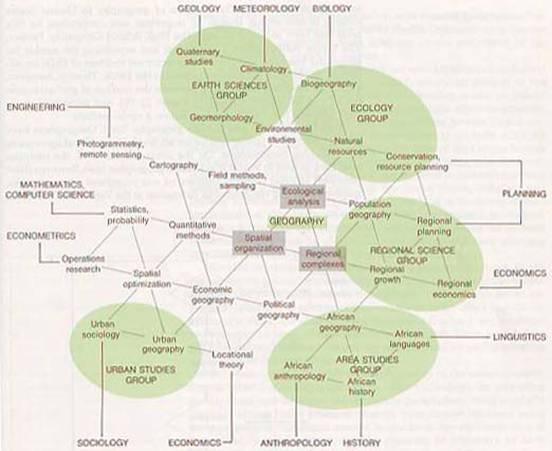
\includegraphics[width=.8\linewidth]{haggett1975_p587.jpg}
    \end{sidecaption}
  \end{figure}

Une exposition des influences de l'écologie, et des sciences naturelles (voir également le schéma \ref{fig:I_geoLink} proposé par \textcite[587]{Haggett1975}), que l'on retrouve beaucoup plus détaillée dans l'étude de l'écologiste et géomorphologue \textcite{Stoddart1967} parue dans \textit{Models in Geography} \autocite{Chorley1967}.

D'un point de vue opérationnel, et c'est aussi le cas dans les précédents ouvrages de ces pionniers, seules des tentatives probabilistes sont évoquées, via les travaux d'Hägerstrand, ou des économistes comme Curry. La méthode hypothético-déductive héritée des premiers géographes théoriciens semble encore être un implicite à la construction et l'évaluation des modèles. Les idées fortes de la systémique semblent avoir été entendues, mais paradoxalement il n'y a à cette période que très peu de références qui se rapportent aux techniques mathématiques ou informatiques capables d’opérationnaliser un tel système, et aucune application réelle \autocite[467-468]{Harvey1969}.

\paragraph{Les pionniers de l'opérationnalisation systémique en Europe}

La génération suivante de géographes va jouer un rôle important dans l'opérationnalisation de ces concepts au début des années 1970, tant en Angleterre, qu'en France où les géographes développent en collaboration avec des mathématiciens et physiciens les aptitudes nécessaires à la manipulation de ces nouvelles techniques computationnelles. \autocite{Pumain2002}

En Angleterre, la planification est issue d'une tradition qui date pour le \textit{Regional Planning and Policy} d'après 1920, et pour le \textit{Land use planning} d'après 1930. Ces activités sont rapidement construites en relations étroites avec les universitaires, les ingénieurs et les politiques publiques \autocites{Bennett2003}[727]{Davies1997}; un existant qui va être bouleversé courant des années 1960-70 par la rencontre conjointe des développements théoriques systémiques, des modèles de planification américains du milieu des années 1950, et d'une littérature qui anticipe la vague systémique. \autocites{Mcloughin1969}[4-8]{McLoughin1985}[253]{Batty1978} \footnote{\foreigntextquote{english}[{\cite[253]{Batty1978}}]{The quantitative revolution in geography as encapsulated in books such as Peter Haggett's (1965) Locational Analysis in Human Geography, the various special issues of the Journal of the American Institute of Planners on traffic (1959) and land-use models (1965), books on the post-industrial structure of cities such as Explorations into Urban Structure (1964) all bolstered and anticipated the systems approach. The second edition of Stu Chapin's Urban Land Use Planning in 1965 was also a land mark in the changing conception of planning in America.}}

C'est sur ce substrat \autocite[253]{Batty1978} que des auteurs comme McLoughlin ou Chadwick publient dès le courant des années 1960 des états de l'art et des manuels d'applications qui vont rester pendant presque dix ans des références pour repenser la planification urbaine sous l'angle nouveau de la systémique \autocite[719]{Davies1997}. Une période qualifiée d'âge d'or pour la systémique anglaise, qui même si elle dure peu de temps \autocites[726-727]{Davies1997}{McLoughin1985}, marque toute une jeune génération de planificateurs qui vont être profondément influencés par ces approches \autocites[5-6]{Batty1976}[256]{Batty1978}; un constat alors en complet décalage avec la situation américaine, qui cristallise comme on a pu le voir dans la section \ref{ssec:crise_mutation} l'échec d'une décennie déjà révolue; les nouvelles pratiques, les nouveaux modèles ayant déjà exfiltrés les Etats-Unis, et la nouvelle génération bricolant déjà les meilleurs modèles en vue de les améliorer. C'est dans ce cadre notamment que le physicien et planificateur Wilson publie en 1970, le résultat de 4 ans de travaux pour concrétiser son idée, passer du paradigme newtonien au paradigme statistique boltzmanien pour revisiter dans une version spatiale et dynamique les modèles numériques classiques américains. \autocite{Wilson2010} Une approche qui va devenir avec le temps \enquote{l'école entropique} comme la nomme \textcite{Guermond1984}.

De cette plus jeune génération, à la croisée de ces inspirations, et tout à fait consciente des errements passés \footnote{Voir la conclusion de l'ouvrage de \textcite[357]{Batty1976} où l'auteur fait le point sur ces différentes positions, toutes abordées en filigrane dans ce livre synthèse : prédiction, explication, éducation }, on trouve des chercheurs maniant parfaitement ces techniques hybrides. Michael Batty est un bon exemple de chercheur représentatif de cette synthèse, qui pressent l'urgence de s'engouffrer dans une modélisation spatialisée plus dynamique \autocite{Batty1971,Batty1972} appuyée par les mathématiques des systèmes dynamiques, que cela soit au travers du vocabulaire de la dynamique des systèmes de Forrester, ou en suivant la toute nouvelle voie des modèles dérivés de l'école entropique de formation par Wilson.

%Le canal en écologie et géographie physique, dans la lignée des travaux de Chorley va également être particulièrement influent, avec l'avénement de modèle opérationel dérivée de la dynamique des populations de Lotka. \autocite{Batty 1971 ou 1972 ....}

%On trouve une analyse des premier essai systémique de Chorley analysé par le prisme des proposition du découpage de Parsons dans l'essai de Gregory.

Comme déjà évoqué brièvement à la fin de la section \ref{sssec:realite_neopositiviste}, les géographes français semblent au début des années 1970 peu réceptifs à l'épistémologie néo-positiviste, et beaucoup plus concentrés sur l'apport des nouvelles méthodes quantitatives dont la substance est révélée brutalement aux géographes français par la lecture (et ensuite la traduction) de manuels anglo-saxons qui condensent déjà 15 ans de pratiques et de découvertes \autocite[129]{Pumain2002}.

Concernant la diffusion du paradigme systémique \footnote{Le cas de la diffusion des méthodes quantitatives en France et de sa structruration en réseau de chercheurs a fait l'objet de la thèse de \textcite{Cuyala2014} dirigée par Marie-Claire Robic, Denise Pumain.}, les recherches d'Olivier Orain \autocite{Orain2001} sur ce sujet sont précieuses. L'auteur nous propose de lister dans les embranchements intellectuels d'une discipline en pleine reconstruction, les convergences et divergences autour de l'acceptation de concepts dont Orain estime qu'ils se sont diffusés dans la géographie française au début des années 1970. La diffusion de la GST de Bertalanffy est renforcée par la publication en 1973 de son ouvrage principal, alors même que l'activité conjointe (publications, traductions, organisations de conférences, d'ateliers) de différents passeurs ayant séjourné à l'étranger comme Bernard Marchand, Wanda Herzog, Henri Reymond, Jean-Bernard Racine, Sylvie Rimbert est soutenue par des acteurs \enquote{installés} comme Philippe Pinchemel, Paul Claval, Roger Brunet, Charles-Pierre Péguy \autocite{Pumain2002,Cauvin2007}, déjà au fait des publications et techniques pionnières anglo-saxonnes.

% NOTE CLEMENTINE et FDD ? il me semble que c’est une des premières thèses françaises dont « système » est le mot clé

Le mot \enquote{système} sort de l'ornière du sens commun et se pare de nouvelles significations, sous l'effet notamment d'ouvrages de référence comme celui de Jean-Bernard Racine et Henri Reymond  \textit{L’Analyse quantitative en géographie} (1973). Premier livre de géographie quantitative en France \autocite{Cauvin2007}, il développe un \enquote{ [...] vibrant plaidoyer pour le développement de concepts et de méthodologies systémistes dans une discipline qui selon eux, \enquote{ découvre que la notion de système lui était depuis longtemps familière, comme la prose à Monsieur Jourdain, et qu'il ne lui manquait que de la formaliser pour la rendre opérationnelle.}} \textcite{Orain2001}. Un appel qui sera entendu semble-t-il, pour Orain \autocite[23]{Orain2001} une des explications pour comprendre le succès connu par la systémique fin des années 1970 début 1980 est le fait que \enquote{[...] les Nouveaux Géographes [...] ont trouvé dans l’idée de système un appareil conceptuel permettant à la fois de penser l’intégration de l’hétérogène et d’apporter une légitimité scientifique à l’étude de la région}.

\Anotecontent{etat_artDPMC}{Sur cette thématique on trouve un excellent récit de Denise Pumain et Marie-Claire Robic \autocite{Pumain2002}, ou de Colette Cauvin \autocite{Cauvin2007}}

Dans l'établissement d'une géographie systémique, le Groupe Dupont qui naît à la suite de la conférence \enquote{révélatrice} donnée par Marchand en 1970 s'avère être un creuset important pour la formation, la réflexion, l'échange intra/inter-disciplinaire, et l'expérimentation autour de ces nouvelles techniques \autocites[2]{LeBerre1987}[125-128]{Pumain2002}. Une structure d'accueil que l'on imagine nécessaire pour fédérer des jeunes géographes plus habitués à l'étude monographique qu'à l'utilisation d'outils computationnels. Une période 1971-1975 marquée par la volonté des \enquote{nouveaux géographes} de se former aux mathématiques, une étape absolument nécessaire pour tirer profit par la suite de ces nouveaux formalismes statistiques et informatiques.\Anote{etat_artDPMC}

% REVUES ÉGALEMENT, voir Pumain2012 (quarante glorieuse de l'espace geographique)

En termes de réalisation, différentes écoles vont se créer autour d'objets géographiques ou de techniques parfois différentes, mais avec la même volonté de rendre compte de la complexité des systèmes géographiques en usant des outils mis à disposition par ce nouveau paradigme systémique. Car ce n'est pas tant l'évolution des concepts qui comptent pour certains géographes mais leur définition en termes opérationnels dans les modèles de simulation \autocite{Pumain2003}, seul moyen de confronter les données récoltées à ces nouvelles formes d'explications mathématiques. Bertalanffy entre autre l'avait déjà bien compris, mobilisées sans réelles démonstrations, les hypothèses intuitées, même lorsqu'elles sont quasi certaines, ne sont tout au mieux pour les autres chercheurs que des aides à la réflexion. Ainsi, et c'est avec une rapidité presque déconcertante, qu'il se raccroche aux premières découvertes de Prigogine en 1946 sur la physique des systèmes ouverts loin de l'équilibre pour appuyer ce qui jusque là ne sont que des intuitions dans sa théorie organismique, et qui forme le prélude à un projet systémique plus général (voir les annexes \ref{sec:annexe} pour plus de détails).

François Durand-Dastès et François Auriac sont des exemples de géographes qui développent dans leurs études toute la puissance heuristique des concepts systémiques et de leur traduction graphique pour décortiquer la complexité des systèmes géographiques.

Un autre groupe de géographes va pousser cette démarche heuristique encore plus loin, en lui donnant corps dans des modèles de simulation. C'est le cas par exemple du projet A.M.O.R.A.L ( Analyse systémique et MOdélisation des ALpes ) réalisé par des géographes et informaticiens grenoblois, qui est un des premiers résultats d'approche systémique spatialisé ayant pour objet d'étude une région française. Un double enjeu et une double expérience ici pour ces géographes, qui décident de tester la méthode systémique en la déroulant dans sa totalité, ce qui signifie également pour les étapes de réalisation de collaborer avec des informaticiens sur la partie système dynamique. \autocite{Guermond1984, LeBerre1987}

\Anotecontent{exp_amoral}{\enquote{[...] mes premières tentatives de modélisation systémique sont liées à un événement conjoncturel : la rencontre de chercheurs en informatique qui travaillaient, dans l'esprit de la dynamique de système de J.W. Forrester, à la mise au point d'un nouveau langage de simulation. Ils cherchaient à identifier, pour les formaliser, les types de problèmes soulevés par les recherches appliquées. Le groupe de géographes grenoblois avec lequel je travaillais, séduit par quelques ouvrages sur l'approche systémique, était tout prêt à faire l'investissement intellectuel pour tenter son expérimentation en géographie. C'est ainsi que nous avons choisi de modéliser la dynamique de l'emploi dans le système urbain de la région Rhône-Alpes.} \autocite[8]{LeBerre1987}}

Dans le cas du modèle A.M.O.R.A.L \autocite{Durand1983}, la démarche poursuivie est explicitement\Anote{exp_amoral} celle de l'expérimentation de l'\enquote{approche systèmes dynamiques} \autocite{Rosnay1975} à l'étude de la région, avec en tête des modélisateurs la réalisation de multiples objectifs, à la fois d'apprentissage, d'amélioration (prise en compte du spatial), de faisabilité, et d'applicabilité décisionnelle.

\Anotecontent{it_allen}{\enquote{Mais la rencontre opérationnelle - décisive -je l'ai faite en 1982, en allant à Créteil écouter - ne me demandez pas pourquoi - un colloque sur l'entropie dans lequel Peter Allen faisait un exposé sur les théories de l'auto-organisation. Dans cet exposé, il décrivait les modalités de changement de ces systèmes ouverts, loin de l'équilibre, qui connaissent de multiples fluctuations, dont certaines pouvaient s'amplifier et contribuer à modifier la structure du système tout autant que certaines bifurcations externes. C'était exactement ce que j'avais observé en étudiant les recensements périodiques de population, en poids économique, et transformaient leur structure qualitative sur le plan de leur portefeuille d'activités économiques, sur le plan de leur composition sociale, tout ceci en lien, bien sûr, avec des représentations que nous avions de cette dynamique des villes en terme d'images de marque, d'attractivité pour les migrations, etc.
Tout de suite j'ai été séduite par cette approche, et j'ai essayé d'expérimenter avec ces modèles mis au point par Peter Allen, qui à l'époque travaillait encore dans le laboratoire de Prigogine à Bruxelles avec Michèle Sanglier, mais plus particulièrement en direction d'applications à l'économie et à la géographie.[...] Il élaborait en effet des modèles spatialisés, notamment un modèle dynamique intra-urbaine ou intrarégionale [...]; il y'avait là beaucoup d'éléments de théories géographiques qui étaient mis dans un modèle de simulation qui permettait d'expérimenter les effets de ces briques théoriques et de les confronter à des observations.} \autocite[153-154]{Mathieu2014}}

\Anotecontent{appli_allen}{\enquote{Tous ces auteurs se sont toutefois heurtés à l'insuffisante prise en compte de la dimension spatiale dans cette famille de modèles. Aussi, des travaux application et élaboration de \textit{modèles urbains} qui soient à la fois \textit{dynamiques et spatiaux} sont en cours. Un modèle comme celui de P.Allen (1978), fondé sur l'analogie des structures dissipatives en physique, permet de simuler le développement d'une ville en tenant compte des interactions non linéaires (avec effets d'amplification ou de saturation), spatiales ou non spatiales, qui commandent la redistribution des emplois et des populations entre les différents quartiers. Il permet de prévoir diverses configurations possibles dans le futur à partir d'une histoire donnée. Ce modèle a été appliqué à la simulation du développement de l'agglomération de Rouen (Ozan et al. 1983)} \autocite{Pumain1983}}

\Anotecontent{auto_definition}{Un autre concept important est introduit par Ashby dans le mouvement Cybernétique, l'introduction du mot \enquote{auto} amorcent un virage réflexif propre à la seconde Cybernétique, pilotée par William Ross Ashby et Von Foerster. Si le concept en lui-même est largement intuité dans les thèses de Goethe et Bertalanffy \autocite[102]{Pouvreau2013} dans sa traduction biologique, on retrouve un concept équivalent dans le \enquote{order-from-noise} de Von Foerster, et \enquote{order-from-fluctuation} dans la physique de Prigogine.}

De façon parallèle, Denise Pumain\Anote{pumain_decouverte}, aidée par d'autres géographes comme Lena Sanders et Thérèse Saint-Julien participe dès 1980 d'un courant \autocites{Pumain1983, Pumain1984, Pumain1989} qui vise l'application des modèles de simulation à l'étude des villes et des systèmes de villes, et cela sur des bases beaucoup plus empiriques, devançant ici les diverses tentatives des anglo-saxons faites jusqu'à alors \autocite[99-100]{Pumain1989}. Mais dans le cas de cette équipe, si l’intérêt porté à la dynamique des systèmes de Forrester est là aussi évidente \autocites{Pumain1983, Pumain1984}, le chemin emprunté sur le plan opérationnel va semble-t-il rapidement diverger de celui suivi par l'équipe AMORAL. Avec la révélation d'une opérationnalisation possible par l'usage de la \enquote{dynamique des systèmes}, les géographes peuvent donc aller plus loin dans l'exploration du support mathématique sous-jacent, et ainsi mesurer dans l'évolution des \enquote{systèmes dynamiques} vue comme discipline mathématique la possibilité de construire des modèles encore plus proches d'une évolution réelle des objets géographiques. Ainsi, là où le modèle AMORAL cherche à spatialiser l'approche systémique qui dérive de la dynamique des systèmes de Forrester, les frustrations de l'équipe de Denise Pumain face à leurs propres études passées sur la dynamique des villes vont les amener à explorer un tout autre chemin en termes d'opérationnalisation.

Ainsi, et c'est dans ce contexte de frustration par rapport aux approches existantes\Anote{appli_allen} que se produit au début des années 1980 cette découverte contingente du concept d'auto-organisation, dont la réalité opérationnelle exprimée dans des modèles mathématiques exposés par les physiciens de l'école de Bruxelles semble offrir tout à coup toutes les garanties pour former des modèles de simulations beaucoup plus réalistes de l'évolution des villes\Anote{auto_definition} \autocite[350]{Pumain1998a}. La possibilité également de concrétiser les intuitions systémiques des pionniers qui envisagent très tôt la nécessité de penser les systèmes urbains comme des systèmes ouverts, comme celle évoquée en 1964 par \textcite{Berry1964a} et son article \enquote{Cities as systems within systems of cities}. La rencontre de Denise Pumain avec le chimiste Peter Allen en 1982 à Créteil\Anote{it_allen} est l'expression même de cette contingence, qui va donner par la suite naissance à de multiples modèles et collaborations avec les physiciens de l'école des \enquote{structures dissipatives} de Bruxelles d'abord, puis de l'école de la \enquote{Synergétique} de Haken ensuite \autocites[27]{Pumain2003}{Pumain1982b, Mathieu2014,Sanders1984, Sanders1992}.

A une phase cybernétique déjà révélatrice de concepts systémiques tout à fait nouveaux pour penser la causalité en géographie, les géographes découvrent par extension la richesse et la pluri-disciplinarité des systèmes dynamiques, alors en pleine évolution. Pourtant déjà évoquées par Poincarré, et étudiées par différents mathématiciens dès le début du siècle, la diffusion des théories de la bifurcation n'atteint son point culminant que courant des années 1970. La conférence de New York en 1977 qui se tient sur ce sujet est selon \textcite{Dahan1991} un marqueur singulier de cette dynamique convergente qui pousse de multiples disciplines (physiques, chimiques, biologiques, etc. ) à se rencontrer, non seulement pour évoquer et mettre en commun leurs questionnements et réflexions sur la nature instable des phénomènes, mais aussi pour venir chercher dans cette conférence de nouveaux outils mathématiques adaptés à sa formalisation. L'apparition de \enquote{systèmes frontières} comme par exemple le système de \enquote{Rayleigh-Bénard} va constituer en devenant un objet d'étude partagé, un formidable point de rencontre entre les points de vue originaux des physiciens développant des appareils de mesures, physiciens, thermodynamiciens, hydrodynamiciens. Mais \enquote{l’adoption d’une approche de type système dynamique pour le comprendre ne constitue pas le moteur principal de la convergence. En fait, l’adoption du langage des systèmes dynamiques est ici plutôt la conséquence d’un désir de convergence manifesté par divers groupes de scientifiques} \textcite{Dahan1991}.

%\begin{framewithtitle}{Les théories de la bifurcation}

	% \begin{figure}[h]
	% \begin{sidecaption}[fortoc]{Un exemple de bifurcation Pitchfork}[fig:S_BPF]
	%   \centering
	%  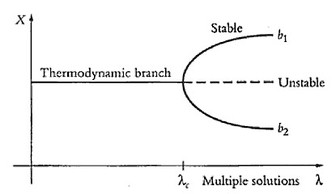
\includegraphics[width=.7\linewidth]{pitchfork_bifurcation.jpeg}
	%   \end{sidecaption}
	% \end{figure}

%\end{framewithtitle}

%La théorie des catastrophe de René Thom, bien connus des géographes, est un cas particulier de la théorie des bifurcations.

Elle offre un support aux découvertes des physiciens engagés depuis les années 1930 dans les travaux sur les processus physiques et chimiques des systèmes ouverts éloignés de l'équilibre, qui observent dans la trajectoire d'évolution de ces systèmes l'apparition de zones d'instabilité, causées par la modification en interne des fluctuations ou en réponse à des variations des échanges externes avec l'environnement.

Si certaines conditions d'une auto-organisation avait déjà été avancées dans une preuve matérielle (Homéostat) et un support théorique (Loi de la Variété requise) dans les travaux par exemple d'Ashby \autocite[800-801]{Pouvreau2013}, les physico-chimistes comme Prigogine ou Haken, en montrant qu'il était possible dans certains systèmes physiques (laser) ou chimiques (structures dissipatives) chaotiques, de voir apparaître au cours des bifurcations de nouveaux équilibres dynamiques caractérisés par l'émergence de structures ordonnées de niveau supérieur issues de l'organisation des interactions à un niveau inférieur, ont fourni une évolution du substrat théorique et mathématique solide du concept d'auto-organisation sur lequel peuvent s'appuyer les chercheurs pour expérimenter des analogies dans les systèmes sociaux ou biologiques.

%l'approche d'un point de bifurcation correspondant à l'émergence d'une structure lié à une variation de paramètres dans un processus chaotique/instable décrivant une trajectoire stable entraînant l'émergence imprévisible d'un nouvel état ordonné/stable, dont la structure est maintenu par consommation d'énergie extérieure.

%dévoile de nouvelle perspectives pour penser l’emboîtement et les relation opérant entre les différentes échelles d'observations (voir Annexe A).

%La matérialisation d'un modèle urbain, même théorique, ouvre la voie à des développements qui ouvre la voie à une nouvelle forme de causalité.

La translation de ces concepts sera opérée avec précaution par Pumain et Sanders, et amène une réflexion sur l'évolution des objets géographiques dont on trouve une plus grande explication dans les textes de \textcite{Pumain1982b, Pumain1989}.

%L'apport du paradigme systémique, et de son opérationnalisation

%Sous détermination
%Equifinalité

%Les deux approches sont clairement supportés par une double dialectique dans l'utilisation des outils statistiques et systémique, et dans la déduction et l'induction. (hum)

%\enquote{Tenant pour légitime de traiter les êtres vivants et leurs associations comme des systèmes physiques, Lotka insistait toutefois sur le fait qu’il s’agit de « systèmes ouverts » aux flux de matière et d’énergie (ainsi que Raymond Defay (en 1929) et Bertalanffy (en 1932) les qualifièrent plus tard), capables d’échapper à l’équilibre thermodynamique défini par un maximum d’entropie promis aux systèmes fermés par le Second Principe, et d’évoluer vers une structuration croissante.}\autocite{Pouvreau2013}

%\autocite{Pouvreau2013} sa théorie arrive à maturation : \enquote{Un système organique quelconque n'est essentiellement rien d'autre qu'un ordre hiérarchique de processus qui se tiennent mutuellement en équilibre de flux [...] Un organisme vivant est un ordre hiérarchique de systèmes ouverts, qui se maintient sur la base de ses conditions systémiques par un changement de ses composants}

%L'apport de ces techniques, est un vrai écho à ce que disait Le Berre; Sanders et Pumain. D'une part les outils permettent d'ouvrir de nouvelles perspectives de réflexions, et ceux ci s’intègrent dans une chaîne de raisonnement qui s'organisent non pas de façon linéaire mais dans dialogue ou ce sont les usages, les questions, les objets à étudier qui guident l'utilisation et l'amélioration de ces outils.

% Partant de Pumain2002 Pumain2003, la première remise en cause de la causalité est le concept de non linéarité des interactions,

% Relation de variété entre les niveau de hierarchie, augmentation du degré de variété, ce qui va avec le concept équifinalité, un peu different du concept de sous détermination...
% Plusieurs débats qui vont venir agiter la problématique de la construction des modèles, et surtout de leur validation.
% Forrester causalité, construction des modèles, sous détermination
% Auto-organisation problématique de

%Dans cette partie, il s'agit donc de mettre en avant ces débats philosophiques en les reliant aux nouvelles problématiques de construction des modèles tel qu'elle apparaissent aux tournant des années 1970.

%Quel sont les moyens offerts de cette validation ? Existe-il une spécificité de cette validation dans son application en science sociale, et plus spécifiquement en géographie, et qui n'est pas prise en compte dans ces définitions ?

%Plusieurs débats viennent encadrer à la fois la validation mais aussi le support opérationel de cette validation. Autrement dit, comment détermine t on si un modèle est validé ou pas, et quel est la nature de cette validation opère sur un substrat particulier, qui en fait une expérience sur le réel de second ordre.

%IMPORTANT : Necessite d'avoir une validation pour les sciences sociales.

\subsubsection{L'impact du programme de Forrester dans le débat sur la Validation}
\label{sssec:forrester_impact}

Deux dates sont à retenir dans le programme forresterien, la publication du \enquote{programme} d'\textit{Industrial Dynamics} en 1961; l'aboutissement des recherches démarrées en 1956 au MIT, et dans un deuxième temps en 1969 la proposition de translation de ce programme à l'étude plus large des systèmes sociaux, avec l'expérience du modèle \textit{Urban Dynamics}.

Pourquoi parle-t-on de programme ici, et non pas seulement de modèle ?

L'apport de Forrester ne se résume pas en réalité au seul nouveau langage de programmation DYNAMO, celui-ci propose aussi avec une méthodologie et un vocabulaire graphique. Trois éléments qui une fois réunis permettent de dériver opérationnellement les concepts clefs du projet systémique dans un modèle de simulation dynamique, ce qui en fait un outil d'intérêt général non seulement pour la géographie, mais pour toute les autres disciplines confondues (biologie, économie, sciences humaines, etc.) \autocite{Rosnay1975}

\paragraph{Urban Dynamics, un révélateur des nouveaux usages pour la construction et la validation des modèles ?}
\label{p:urbanDyn_revelateur}

Provenant d'une toute autre inspiration et construit selon un tout autre patron que les modèles urbains réalisés jusqu'à la fin des années 1970, le modèle \textit{Urban Dynamics} de \textcite{Forrester1969} fait une entrée très remarquée dans le milieu des \textit{policies}. Celui-ci met en jeu une ville abstraite et isolée, non-spatialisée, où interagissent de façon a-spatialisée de multiples mécanismes regroupés par activités et organisés en chaîne causale. Le modèle ne fait appel à aucune donnée pour calibrer ou vérifier les sorties générées, et à ce titre il ne peut pas être considéré comme un modèle décisionnel sérieux pour les \textit{policy analysis} de l'époque. \autocite{Lee1973}. Soumis à une très forte médiatisation, les critiques sur le modèle se font parfois vives tant du côté des citoyens \autocites{Forrester1989, Forrester2007} que des universitaires géographes \autocites{Tobler1970a, Berry1970b, Batty1971, Batty1976} .

Il est vrai que d'un point de vue purement géographique et même technique, le modèle \textit{Urban Dynamics} n'introduit pas tant d'originalité par rapport aux éléments acquis par la rencontre entre la vision d'Hägerstrand et les pionniers universitaires 10 ans auparavant. On se remémorera à ce sujet la citation de \textcite{Morril2005} qui résume très bien l'importance de cette convergence, ici en quatre grands points : \foreignquote{english}{First was the introduction (at least at the geography) of the idea of spatial and time-processes, that geographic development over time could be understood and modeled; second was the particular processes of spatial diffusion; third was the technique of Monte-Carlo simulation; and fourth was the idea that individual behavior, not just that of large groups, could be modelled}. Ainsi après tout, les premiers modèles de simulation qui incorporent la dimension temporelle, stochastique, dans le premier langage Fortran, sont datés d'avant 1965, et dépassent en bien des aspects la vision a-spatiale proposée par Forrester.

L'étude des processus de diffusion abordés dans les simulations pionnières suppose assez naturellement que les géographes intègrent le temps dans leurs analyses, et il a été vu précédemment que la simulation est un formidable outil d'expérimentation pour la projection et l'évaluation dans le temps de multiples hypothèses (section \ref{ssec:labo_virtuelle}). En dehors de quelques exceptions\Anote{batty_temps}, pourquoi cette approche percole-t-elle aussi lentement dans l'analyse des systèmes urbains en géographie, où la simulation numérique est mobilisée à la même période sans pourtant y intégrer la dimension temporelle? Sorte de principe de parcimonie poussé à l'extrême, où l'absence du temps si elle permet de simplifier l'analyse, mène toutefois à des prédictions absurdes ou impossibles, qui ne tiennent pas compte des évolutions de structures sur lesquelles s'appuient les interactions dans les systèmes urbains. Le constat d'une forme d'auto-censure de la discipline pour laquelle \textcite[296-297]{Batty1976} nous donne quelques pistes de compréhension :

\foreignblockquote{english}[{\cite[296-297]{Batty1976}}]{There are, however, good reasons why the comparative static approach has been widely applied. The status of theory in urban economic and geographic systems with regard to time is almost non-existent. [...] Yet there are severe problems in trying to develop dynamic theory, two of which are worthy of some discussion.[...]

Perhaps the major problem concerns the ability to observe or monitor the urban system. Unlike the physical sciences in which the effect of critical variables on the system of interest can be isolated in the laboratory, such a search for cause and effect is practically impossible in social systems. Thus, there are many instances when it is difficult, if not impossible, to disentangle one cause from another in the changing behaviour of such systems. This is a fundamental limitation which is referred to here as the \textbf{observational dilemma}.

A second problem concerns that hoary perennial data. [...] data are often difficult to assemble for one cross-section in time, and the collection of time series data is usually a formidable and sometimes infeasible undertaking. Furthermore, such data often become less consistent and sparser as earlier time periods are needed and, frequently, the time periods between points at which data have been collected, are too large to be useful for dynamic modelling}

%%NOTE CLEMENTINE à ce propos, pour préparer mon entretien skype, j’ai regardé plein de vidéos récentes de Batty et de son accent bien anglais. Y’en avait une je sais plus où assez cool qui répond à cette citation de 40ans. En gros, il parle des Big Data et de la façon dont leur structure (non-exhaustif, irrégulières dans le temps mais dans un temps plus ou moins continu etc.) change qualitativement les analyses. C’est pas juste plus de données mais données différentes et questions à poser d’un autre ordre. juste comme ça.

Si on revient au modèle \textit{Urban Dynamics} de Forrester, celui-ci pourrait après tout passer pour une nouvelle tentative parmi d'autres, car comme Tobler le fait remarquer dans sa critique du modèle : \foreignquote{english}{In other words, it is a classical non-linear deterministic equilibrium model, but of great complexity.} \textcite{Tobler1970a}

Pourquoi Batty en fait-il alors régulièrement un modèle pivot dans son argumentation dans l'évolution de la discipline \textcite{Batty1971, Batty1976, Batty2001, Batty2008}, et pourquoi celui-ci a-t-il autant attiré l'attention dans le monde académique ?

Sur ce deuxième point, on a déjà donné un élément de la réponse dans l'introduction de cette partie. Forrester vient ici avec plus qu'un modèle, il vient avec un programme \autocite{Forrester1961} qui embrasse littéralement les concepts de la systémique dans sa branche cybernétique \autocite{Berry1970b}, ce qui permet d'apporter, avec l'intégration du temps, un tout nouveau point de vue sur la planification et la mise en place des politiques publiques. Ainsi malgré ses défauts, \foreignquote{english}{[...] the model is an illustrative first attempt that points the way for others. It is the direction that is important, and Forrester's book may yet prove to be one of the important signposts in the attempt to deal more sensitively and effectively with urban problems.} \autocite{Berry1970b}

L'autre point fort du programme de Forrester est la possibilité d'opérationnaliser des concepts de la systémique tout en maintenant un coût d'accès à la simulation qui paraît plus adapté au monde académique des sciences humaines et sociales, et cela entre autre par la mise en place d'une triple entrée en la matière : informatique avec DYNAMO (un langage déjà adapté/simplifié pour réaliser des simulations), mathématique avec les systèmes dynamiques, et graphique avec les diagrammes de \foreignquote{english}{stock and flow}.

%NOTE CLEMENTINE une figure-exemple ?

Pour ces deux raisons, on comprendra donc ici que le monde académique soit plus intéressé par les nouvelles possibilités offertes par l'environnement support du modèle que par le modèle en lui-même, qui restera chez les géographes un cas d'utilisation finalement assez peu repris dans des travaux ultérieurs chez les anglo-saxons \autocite[308]{Batty1976}, et chez les français. %\hl{(ref)}

Ainsi, ce n'est pas tant sur les aspects temporels que \textcite{Batty2001} en font un modèle en rupture avec son passé, mais sur le débat qu'il soulève du point de vue de la validation.

\foreignblockquote{english}[\cite{Batty2001}]{Perhaps the clearest model which broke from this tradition and which illustrated distinctly the problems posed by the current generation of models based on complexity was Forrester’s (1969) Urban Dynamics model.} \autocite{Batty2001}

Pour comprendre la position de Forrester sur ce point il faut s'intéresser d'un peu plus près à sa vision de la modélisation et à l'utilisation qu'il souhaite en faire dans le cadre des politiques publiques. Pour lui, le problème n'est pas tant les données, que l'on finit toujours par obtenir, \foreignquote{english}{ [...] but rather inability to perceive the consequences of information we already possess.}\Anote{batty_donnees}\Anote{batty_ok}. Les décideurs politiques se font une image de la réalité - modèle mental -, or souvent cette image serait trompeuse, ce qui amèneraient à la faillite des politiques ainsi menées. Pour \textcite{Forrester1971}, l'usage de modèle de simulation permet de re-projeter ces modèles mentaux faillibles sur des modèles informatiques dont la construction nécessite la formulation d'hypothèses de façon plus explicite, plus compréhensible, et sur lequel il est possible de dialoguer de façon plus constructive. Il n'est plus question de choisir en fonction d'un seul scénario, mais de plusieurs, avec la possibilité de projeter et d'évaluer dans le temps les conséquences de dynamiques complexes sur un système simplifié envers un objectif donné, et cela avec la garantie d'une fiabilité bien au-delà de ce que le seul esprit humain ne pourrait espérer. Avec souvent un résultat sans appel, \foreignquote{english}{[...] behavior is different from what people have assumed.} Un comportement qu'il arrive à démontrer par le jeu des rétro-actions des mécanismes de son modèle \textit{Urban Dynamics}, qui illustre les effets tout à fait contre-intuitifs de certaines politiques publiques.

Comme sous-entendu dans le paragraphe précédent, en réalité on comprend beaucoup mieux la démarche de Forrester dès lors qu'on comprend qu'il n'a jamais été question ici de faire un modèle opérationel, comme le sous-tend aussi \autocite{Batty2001} : \foreignquote{english}{It might be, as was argued at the time, that the purpose of this model was to raise the level of debate about the inner city. It was not to provide an operational simulation. It was to foster discussion about possible policy issues.}

Ce qui explique entre autre la curiosité ou la perplexité des planificateurs \autocite{Lee1973} ayant investi des millions de dollars sur plusieurs dizaines d'années dans la construction de modèles s'appuyant sur des récoltes de données à la fois coûteuses et fastidieuses.

Le support de cette discussion passe par l'établissement d'un graphe causal représentatif d'un système clos dans sa définition, mais ouvert dans ses échanges vers l'extérieur, dont les éléments et les interactions entre les éléments sont au centre du débat. %\hl{description graphe forrester}

Mais en acceptant cela, et compte tenu de l'\textit{observational dilemna} défini par Batty, le modèle de simulation devient dans l'établissement de sa structure causale la projection d'une histoire, d'un point de vue, ici celui de Forrester et de ses collaborateurs. Dès lors l'attention ne se porte plus seulement sur le résultat, mais aussi sur le bien fondé des hypothèses mobilisées par Forrester pour établir ce résultat.

Il y a un certain paradoxe à voir dans cette situation, car si effectivement Forrester donne à voir avec ce graphe causal son raisonnement, contrairement à de nombreux modèles urbains autrefois qualifiés de \enquote{boîte noires}, c'est précisément sur ce point qu'il va se faire attaquer. Les critiques des géographes ne manquent pas alors de rappeler qu'en dehors de l'a-spatialité et l'isolation du modèle, celui-ci n'a intégré absolument aucune référence aux théories urbaines dans son travail. Outre, le fait que ce n'est pas très \textit{fair play} de sa part pour les universitaires travaillant sur ce sujet depuis 10 ans, cet isolement relatif (Forrester mobilisera d'autres sources) se traduit dans le modèle par la mise en oeuvre de centaines d'hypothèses (400 équations, 300 variables et paramètres \autocite[63]{Pumain1989}) qui s'avèrent pour la plupart difficilement justifiables ou testables de façon empirique \autocite[307]{Batty1976}.

La critique de \textcite{Tobler1970a} sur ce point est explicite, \textit{Urban Dynamics}

\foreignblockquote{english}[\cite{Tobler1970a}]{[...] is a classical non-linear deterministic equilibrium model, but of great complexity. Herein lies its importance for it is rather grandiosely conceived. [...] Not only the values of the parameters, but also which variables are chosen for consideration and how they are interconnected, are critical. [...] the danger is that his model has not really been tested empirically, thus the policy implications may be wrong, and the model - because of its complexity - is extremely difficult to test. A very careful study of the many assumptions of the model are required. Also required are more competing models, thus the book’s greatest achievement may be the competition which it stimulates.}

Dernier point, peut-être le plus préjudiciable à la démarche vantée par Forrester, est la règle qu'il donne pour définir le choix des hypothèses dans un graphe de causalité :

\foreignblockquote{english}[\cites{Forrester1968b, Richardson2011}]{Formulating a model of a system should start from the question \enquote{Where is the boundary, that encompasses the smallest number of components, within which the dynamic behavior under study is generated?} [...] In concept a feedback system is a closed system. Its dynamic behavior arises within its internal structure. Any action which is essential to the behavior of the model being investigated must be included inside the system boundary.}

Sachant cela, et le fait que différentes équipes arrivent à reproduire la même dynamique finale avec la mise en œuvre de modèles beaucoup plus parcimonieux, l'effet est catastrophique pour l'argumentation de Forrester ! Lee\Anote{lee_forrester} et Batty\Anote{batty_forrester} font référence en particulier aux travaux de \autocite{Stonebraker1972}.

Ainsi quand \textcite{Batty2001} parlent du modèle de Forrester comme ayant polarisé le débat, ce n'est pas pour éclairer sa réussite dans cette lourde tâche de fabriquer un modèle crédible sur le plan des hypothèses du point de vue d'une communauté des géographes, car sur ce point l'échec semble complet. Son approche légitime par contre indirectement une construction de modèles complexes qui n'impliquent pas forcément une vérification stricte par les données (sur les hypothèses, mais aussi en sortie). Une \foreignquote{english}{Forrester strategy}, identifiée par \textcite[7-8]{Batty2001} comme le retranchement des modélisateurs dans une rhétorique masquant en réalité une absence de volonté ou une incapacité (technique, méthodologique, philosophique) à justifier de la chaîne causale mise en place dans le modèle, celui-ci ne servant plus qu'à animer ou illustrer un débat où clairement la neutralité scientifique n'est plus une priorité.

Le débat s'organise alors autour d'un problème qui parait insoluble, avec d'un côté cette nécessité - pour être crédible d'un point de vue scientifique - de pouvoir justifier empiriquement le réseau d'hypothèses mobilisées dans notre modèle complexe, et d'un autre côté l'impossibilité de pouvoir toutes les justifier du fait de l'\textit{observational dilemna} et de la difficulté/impossibilité d'obtenir des données dans bon nombre de disciplines en sciences sociales. Un paradoxe d'autant plus renforcé quand on sait que la simulation est justement mobilisée dans certaines disciplines pour mettre en valeur des comportements du système jugés inobservables dans la réalité, soit parce que qu'ils ne peuvent pas être isolés, soit parce qu'ils ont tout simplement disparus.

Remis dans son contexte, et bien qu'elle soit affaiblie justement par le choix d'une cible plus politique (une réussite pour avoir montré qu'il y a des phénomènes contre-intuitifs) que scientifique (un échec du point de vue des hypothèses injectées), la thèse de Forrester a le mérite de se positionner comme une validation avant tout dépendante d'un contexte. Un point de vue qui peut paraître évident aujourd'hui mais qui va pour l'époque se heurter à une vision de la validation héritée de l'économie beaucoup plus rigide sur ce point de vue, et dont nous allons voir qu'elle est de toute façon inadaptée à la validation des modèles en sciences sociales.

%Car comment valider un modèle qui ne s'appuie sur aucune données autres que des valeurs de paramètres, et qui évoque des conclusions sans avoir été calibré au préalable ? Comment discuter des résultats de cette longue suite d'hypothèses reliés les uns aux autres par des interaction complexes, difficile ou impossible à vérifier empiriquement ? On retrouve là les deux points évoqués par Batty pour justifier du retard dans l'intégration du temps dans les modèles urbains, sur lesquels Forrester est clairement mis en difficulté.

\paragraph{Forrester, un acteur du débat entre Validation Objectiviste et Relativiste}
\label{p:confrontation_approches}

Avant même la publication de \textit{Urban Dynamics}, c'est déjà sa première publication \textit{Industrial Dynamics} qui doit faire face à plusieurs critiques extrêmement vives de la part d'opposants à sa méthode de validation \autocite{Barlas1990}. Ces derniers affichent alors des vues plus proches d'une autre méthode de validation, beaucoup plus rigide, telle qu'elle est proposée par Naylor; un des pionniers sur cette question et dont la vision a une large influence dans la littérature de la validation courant des années 1960-1970. Un postulat qui se base à la fois sur des commentaires de chercheurs comme \autocite[1088]{Kleindorfer1998} \autocite{Nance2002}, mais également d'une constatation faite dans la lecture des ouvrages collectifs \autocite{Guetzkow1972}, où Naylor apparaît souvent comme la voix référente sur cette question.

Bien que sa méthodologie soit la plus souvent citée dans le domaine de la \textit{V\&V} comme une \enquote{méthodologie historique} \autocite{Sargent2010}, celle-ci reste pourtant tout à fait influente et opérationnelle de par sa présence régulière dans des ouvrages d'ingénierie généraliste. \footnote{Jerry Banks dans son livre régulièrement réédité \textit{Discrete-Event System Simulation} propose toujours aux lecteurs de valider leur modèle en s'appuyant sur une version synthétique et modernisée de l'approche proposée par Naylor}

Pour \textcite{Kleindorfer1998}, cette vision historique de la validation telle qu'elle a été définie par Naylor est la cause encore aujourd'hui de nombreux malentendus et critiques qui touchent la validation de modèles. A ce titre, et dans le but de faire progresser ce débat, \textcite{Kleindorfer1998} se positionne comme arbitre entre d'un côté l'\enquote{objectivisme} représenté par Naylor, et de l'autre côté la vision opposée plus \enquote{relativiste} représentée par Barlas et Carpenter, eux aussi extrêmement critiques envers la vision de Naylor.

Une fois remise dans son contexte, la méthodologie proposée par Naylor est au premier abord particulièrement intéressante; pas seulement car c'est la première fois que l'on s'intéresse à cette problématique, mais aussi parce que celle-ci aborde cette réflexion en y intégrant spontanément le point de vue de la philosophie des sciences. Mais il ne s'arrête pas là, car c'est avec une certaine ouverture d'esprit qu'il insiste ensuite auprès du lecteur sur la nécessité d'une approche éclectique de cette question de la validation; celle-ci n'étant pas pour lui l'histoire d'un seul dogme forcément incomplet, mais d'un faisceau d'approches résolument complémentaires. Il retient trois approches qu'il regroupe par ordre d'application dans une méthode nommée \textit{Multi Stage Validation} et qui contient : le rationalisme cartésien, l'empirisme, et la \textit{positive economics} de Friedman.

Seulement, après lecture et analyse de cet article, on s'aperçoit que les trois points de vue qu'il présente se rapportent à une vision de la validation en réalité assez rigide, comme en témoigne cette citation tirée de l'article de \textcite{Naylor1967} : \foreignquote{english}{To verify or validate any kind of model (e.g management science models) means to prove the model to be true. But to prove that a model is \enquote{true} implies (1) that we have established a set of criteria for differentiating between those models which are \enquote{true} and those which are not \enquote{ true }, and (2) that we have the possibility to apply these criteria to any given models}

Pour \textcite{Barlas1990, Barlas1996}, il existe deux camps philosophiques opposés, et pour lui Naylor fait clairement partie de la première école :

\foreignblockquote{english}[\cite{Barlas1990}]{The traditional reductionist logica1 positivist school (including empiricism, rationalism, verificationism and the “strong” falsificationism) would see a valid model as an objective representation of a real system. The model can be either “correct” or “incorrect”; once the model confronts the empirical facts, its truth or falsehood would be automatically revealed. In this philosophy, validity is seen as a matter of accuracy, rather than usefulness. The opposing school (including more recent relativistic, holistic and pragmatist philosophies), in contrast, would see a valid model as one of many possible ways of describing a real situation. \enquote{No particular representation is superior to others in any absolute sense, although one could prove to be more effective. No model can claim absolute objectivity, for every model carries in it the modeler’s worldview. Models are not true or false, but lie on a continuum of usefulness}.}

\textcite{Barlas1990} font de Forrester le premier défenseur d'une validation plus en accord avec la deuxième école, une méthode selon lui plus adaptée à l'explication de processus complexes, comme en témoigne ces quelques extraits tirés de son article :

\foreignblockquote{english}[\cite{Barlas1990}]{The first exposition of the system dynamics paradigm as it relates to model validity was given in Chapter 13 of Industrial Dynamics (1961) by Jay Forrester. [...]

Forrester also criticizes the illusion that using fixed statistical significance levels brings objectivity to the validation procedure. [...]

He makes the stronger claim that \foreignquote{english}{the validity of a model should not be separated from the validity and the feasibility of the goals themselves.} Since reaching an agreement on the feasibility of the goals cannot be achieved through a formal algorithmic process, validation becomes very much a matter of social discussion. [...]

Another nontraditional view of Forrester is his willingness to accept \foreignquote{english}{qualitative} model validation. He argues that a negative attitude toward qualitative validation procedures is not justifiable, since \foreignquote{english}{a preponderant amount of human knowledge is in nonquantitative form} \autocite[128]{Forrester1961}. [...]

Finally, Forrester sees explanatory power as being at least as important as predictive power in model validation. Forrester’s views on model validity correspond to the relativist/holistic philosophy of science. }

En ce sens il prend le contre-pied de la dernière méthode qui clôt la \textit{multistage validation} de Naylor. La \textit{positive economics} dictée par Friedman, une forme d'instrumentalisme, est complétée par les deux méthodes précédentes (empirisme, rationalisme) pour assurer que la validation du modèle, et des hypothèses qu'il contient, est bien dirigée en priorité par la prédiction : \foreignquote{english}{ Hence the final decision concerning the validity of the model must be based on its predictions.} \autocite[97]{Naylor1967} Or il a été montré précédemment (voir \ref{p:echec_critiques} que c'est bien un des points reprochés par une partie des géographes radicaux que de voir s'aligner une partie des géographes (volontairement ou involontairement) sur une forme d'instrumentalisme, hérité de l'économie, et cela même appuyé par une position empiriste pour la validation des hypothèses.

Clairement le paradigme systémique permet d'échapper à ce discrédit par l'intégration dans les modèles géographiques d'une réflexion à la fois multi-échelle, et multi-temporelle \autocite{Dastes2001a} dont la discrétisation en une multitude de points d’arrêt pertinents constitue il me semble un appel implicite à l'étude inter-disciplinaire des objets géographiques, et dont la collection est toujours abordée en fonction de la question qui est posée. Ainsi l'étude de l'évolution comparée des systèmes de villes dans le temps long, ou l'étude des mobilités des individus liés à l'attribution des cartes scolaires sont deux exemples de sujet dont les composantes complexes ne peuvent être abordées sans faire appel à l'expertise comparée de sociologues, d'archéologues, d'économistes, etc. qui disposent pour le même objet (l'individu, la ville) de points de vue prompts à enrichir les modèles d'une hétérogénéité permise par la systémique.

Autre point qui semble en divergence avec les pratiques des géographes, la position empiriste de Naylor implique de limiter le choix d'hypothèses mobilisées dans les modèles aux seules qui peuvent être validées par des données : \foreignblockquote{english}[\cite{Naylor1967}]{A simulation model, the validity of which has not been ascertained by empirical observation, may prove to be of interest for expository or pedagogical purposes, but such a model contributes nothing to the understanding of the system being simulated}

Une vision radicale qui se heurte au problème de l'induction comme il avait déjà été évoqué pour les positivistes logiques ( section \ref{p:critique_debat} ), l'accumulation de confirmation n'étant en aucun cas une condition suffisante à la validation d'une hypothèse.

De plus, toutes les disciplines n'ont pas la possibilité de disposer de données utilisables pour vérification des hypothèses, et d'autre part la collecte et la structuration des données tient d'un processus qui contient là aussi une part de choix qui rend discutable la mise en place d'un seul jeu d'observation pour validation d'une seule et même hypothèse.

Enfin, cette vision est de toute façon peu compatible avec une étude de la complexité des systèmes sociaux (\foreignquote{english}{observational dilemna} de Batty), car comment rendre compte par une récolte de données de processus dont on sait d'une part que la perception et donc l'établissement de mesure est subjective (voir point précédent) et d'autre part que ces processus ne peuvent être réduits à leur seule composante du fait de leur intrication dans un réseau complexe d'interaction (le tout est plus que la somme des parties).

%Cela pour plusieurs raisons qui tiennent à la construction des connaissances dans la simulation des systèmes sociaux, dont on verra par la suite qu'elle ne peut que difficilement être similaire à la construction des connaissances dans les sciences naturelles.

%La où la validation proposée par Naylor ne se réalise en effet qu'à l'aune des données disponibles, et se rapproche dans sa description plus d'un résultat binaire propre au cadre d'évaluation des positivistes logiques; Forrester propose avec l'établissement d'un graphe causal l'intégration explicite du social, du contexte dans lequel se construit, et donc se valide le modèle.

Toutefois, et avant de rejeter l'une ou l'autre approche de façon hâtive, on citera \textcite{Kleindorfer1998} pour résumer quelles sont les conséquences pour le raisonnement d'un modélisateur qui veut s'en tenir à la stricte application d'un de ces deux pôles. Ainsi un objectiviste extrême \foreignquote{english}{[...] believes that model validation can be divorced from the model builder and its context. He or she maintains that models are either valid or invalid, and that validation is an algorithmic process which is not open to interpretation or debate.} alors que par contraste un relativiste extrême \foreignquote{english}{[...] believes that the model and model builder are inseparable. As such, all models are equally valid or invalid and model validity is a matter of opinion.}

Évidemment intenables en tant que tels, ces extrêmes portent en chacun d'eux une part de vrai qui les rendent tous deux intéressants. Pour \textcite{Kleindorfer1998} en réalité la plupart des scientifiques intègrent spontanément l'une et l'autre de ces approches dans leurs pratiques de validation.

\foreignblockquote{english}[{\cite[1098]{Kleindorfer1998}}]{Objectivism seeks a common framework with which to evaluate and compare models and a sense in which the validation process transcends the model builders and users. By contrast, the relativist position highlights the need for a dialogue between the model builder and other model stakeholders. According to \autocite{Barlas1990}, validation is \enquote{a matter of social conversation rather than objective confrontation.} We would argue that most practitioners have instinctively adopted a middle ground in this debate.}

Attention donc ici à ne pas se tromper de cible, \textcite[188]{Barlas1996} en lui-même ne rejette pas les méthodes quantitatives, pas plus que Forrester, seulement il met en avant le fait que la procédure de validation ne peut se limiter à une validation totalement objective, universelle, quasi-algorithmique et blâment le fait qu'on puisse penser l'explication au seul terme des prédictions qu'elle est susceptible d'apporter.

Dans son travail d'établissement d'une typologie autour des termes sur la validation, \textcite{Augusiak2014} résume le point de vue de ces auteurs ainsi :

\foreignblockquote{english}[\cite{Augusiak2014}]{Barlas and Carpenter (1990) as well as Oreskes and Belitz (2001) and Oreskes et al. (1994a) argue that one such representation may be preferable over other alternatives, but that no model could claim absolute objectivity as each is also subject to the modeller’s subjectivity, view and understanding of the world, and proneness to mistakes. Thus, models are neither true nor false but lie on a continuum of usefulness for which credibility can be built up only gradually (Barlas and Carpenter, 1990; Rykiel, 1996). The question is transferred from whether or not a model holds true to how likely it is to be sufficiently true in the light of accumulated, existing evidence and the model’s purpose.}


% REVOIR TRANSITION
%Dès lors on est en mesure de poser la question suivante, quels sont les modalités de cette nouvelle forme de validation proposés par Forrester ?

%PEUT VENIR EN SOUTIENT DE LARGUMENTATION, EN EXEMPLE.
%\paragraph{Forrester, ou les moyens de cette discussion}
% PERMET DE FAIRE EMERGER UN GRAPHE CAUSAL
% PERMET DE FAIRE EMERGER L'IMPORTANCE DU COLLECTIF

%En cela il répond déjà à une des critiques majeures faites aux anciens modèles, composés

% problématique de la tension entre l'objet construit, et l'objet à valider, car la validation on va le voir est le propre à la fois d'une discussion interne mais également externe avec le reste du monde. (du coup il faut aussi développer les moyens, et ca sera la la transition dans la conclusion)

Bien que reconnu comme pionnière, l'approche de Naylor n'est pourtant pas la seule à émerger dans le courant des années 1960-70 \autocite{Balci1980}, ainsi on a vu par le biais de \autocite{Barlas1990} que Forrester disposait déjà en 1961 d'un avis suffisamment tranché pour s'opposer à cette dernière. En étudiant les textes de \textcite{Hermann1967}, on découvre un autre pionnier de la \enquote{V\&V}, opérant cette fois-ci dans un tout autre contexte de modélisation que Naylor. On se rend compte que le discours développé par Hermann est d'une toute autre nature. Tout en étant compatible avec le discours de Forrester sur la nature contextuelle de la validation, celui-ci va plus loin en proposant à la fois une réflexion et des solutions - dont une large partie a été intégrée dans les synthèses successives et ultérieures du mouvement de la \enquote{V\&V} - sur des problématiques qui résonnent encore, à la mesure de nos travaux actuels, comme étonnamment contemporaines.
